\documentclass[a4paper,11pt]{book}
\usepackage[T1]{fontenc}
\usepackage[francais]{babel}
\usepackage{biblatex}

\usepackage[top=2.0cm, bottom=3cm, left=2.5cm, right=2.5cm]{geometry}
\usepackage{graphicx}
\usepackage{wrapfig}
\usepackage{amsmath,esint}
\usepackage{amssymb}
\usepackage{esvect}
\graphicspath{{figures/}{../figures}}
\usepackage{fancyhdr}
\usepackage{lastpage}
\usepackage{hyperref}
\usepackage{mdframed}

\AtBeginDocument{
\addtocontents{toc}{\protect\label{toc}}}

\newcommand*\dif{\mathop{}\!\mathrm{d}}
\newcommand*\diver{\mathop{}\!\mathrm{div}}
\newcommand*\grad{\mathop{}\!\mathrm{grad}}

\title{Exercices de colle - seconde année de CPGE - MP/PC/PSI}
\author{Matthieu Santin}

\pagestyle{fancy}
\renewcommand\headrulewidth{1pt}
\fancyhead[L]{Exercices de colles}
\fancyhead[R]{Matthieu Santin}
\fancyfoot[C]{\thepage/\pageref{LastPage}  \hyperref[toc]{$\uparrow$}}
\fancyfoot[R]{}

\mdfdefinestyle{stylecorrection}{%
middlelinewidth=0pt,
roundcorner=1pt,
backgroundcolor=seagreen,
innerleftmargin=5pt,
innerrightmargin=5pt,
leftmargin=0pt,
rightmargin=0pt,
skipabove=0pt}

\definecolor{seagreen}{RGB}{215,244,238}
\newenvironment{correction}
{\noindent\begin{mdframed}[style=stylecorrection]
%\begin{small}
\small\setlength{\parindent}{0pt}
\noindent\textit{\textbf{\underline{Corrigé} :}\newline}
}
{%\end{small}
\end{mdframed}
}

\begin{document}
\frontmatter
%\begin{center}
The front cover
\end{center}
\maketitle
%\begin{center}
\large
For \ldots
\end{center}
\begin{center}
Les exercices proposés dans ce document sont issus d'exercices de concours, d'exercices classiques de CPGE ou de mon imagination. 
\end{center}
\tableofcontents
%\chapter{Preface}
The preface text. See \cite{doody}.

% =========================
\mainmatter
\chapter{Electronique}

\newpage

\section{Puissance consommée par un AO $\bullet\circ\circ\circ$}
 
On souhaite alimenter un dispositif électrique (en rouge) modélisé par une résistance de charge $R_c$ avec une tension nominale $V_{nom}$. On dispose pour cela d'une source de tension (en bleue) mais dont la tension de sortie maximale $V_{max}$ est $V_{max} = V_{nom}/2$, insuffisante pour l'usage voulu. On introduit un montage intermédiaire pour compenser l'insuffisance de la source. 

\begin{figure}[!h]
\centering
\includegraphics[width=0.5\linewidth]{electronique_puissance_AO.pdf}
\end{figure}

\begin{enumerate}
	\item Calculer $U_s$ en fonction de $U_e$ et déterminer le rôle de ce montage. Comment doit-on choisir $R_1$ et $R_2$ pour que $U_s = V_{nom}=2V_{max}$ ?
	\item On suppose dans un premier temps que $R_c=\infty$, cad que la résistance de charge n'est pas connectée au circuit. Quelle est la puissance électrique émise par l'AO ?
	\item On suppose maintenant que le circuit est connecté à la charge, cad que $R_c$ est finie. Quelle est désormais la puissance dégagée par l'AO ?
	\item Comment choisir $R_1$ et $R_2$ de sorte à minimiser la puissance sortie par l'AO ?
\end{enumerate}

\newpage

\begin{correction}

\begin{enumerate}
	\item Amplificateur non-inverseur $u_s = \frac{R_1+R_2}{R_2}u_e$. Pour que $U_s = V_{nom}=2V_{max}$ il faut que le montage double la tension, cad $R_1=R_2$.
	\item  Si $R_c=\infty$, alors le courant dans la charge $i_c$ est nul. Alors $P=u_si_s= \frac{R_1+R_2}{R_2^2}u_e^2$. L'AO consomme de l'énergie même s'il n'y a aucune puissance délivrée à la charge !
	\item Soit $i_1$ le courant traversant $R_1$ et $R_2$. Alors la loi des nœuds donne : $i_s-i_1-ic=0$ (signe pris tq les puissances soient positives). On a alors :
	\begin{equation}
		P=u_si_s=\frac{R_1+R_2}{R_2^2}u_e^2+\frac{(R_1+R_2)^2}{R_2^2R_c}u_e^2
	\end{equation}
	\item On prend $R_2\gg R_c$, le premier terme de dissipation de l'AO devient négligeable devant la puissance envoyée à la charge.
\end{enumerate}

\end{correction}

\newpage

\section{Montage passe-bas $\bullet\bullet\circ\circ$}

On considère le montage suivant. L'ALI est supposé idéal.

\begin{figure}[!h]
\centering
\includegraphics[width=0.5\linewidth]{electronique_circuit_6.pdf}
\end{figure}

\begin{enumerate}

	\item Montrer que la fonction de transfert de ce filtre s'écrit sous la forme :
\begin{equation}
	H=H_0\frac{1+j\omega/\omega_0}{(1+j\omega/\omega_1)(1+j\omega/\omega_2)}
\end{equation}
On donnera l'expression de $\omega_0$, $\omega_1$ et $\omega_2$.

\item Tracer le diagramme de Bode correspondant en fonction des différentes pulsations en jeu. Expliciter les cas possibles.

\item On considère désormais que $R=R_1=R_2$ et $C_1=C_2=C$. Simplifier la fonction de transfert, en introduisant $\omega_0=1/RC$. A quel type de filtre à t-on affaire ?

\item On envoie en entrée le signal suivant :
\begin{equation}
	U_e(t) = \frac{4U_0}{\pi}\sum_{p=0}^{\infty}\frac{1}{2p+1}\sin(2(p+1)\omega t)
\end{equation}
On suppose que $\omega\gg\omega_0$. Quel est le signal de sortie $U_s$ ? Donner son allure et commenter. 

\end{enumerate}

\newpage

\begin{correction}

\begin{enumerate}

	\item Fonction de transfert :
\begin{equation}
	H=\frac{u_s}{u_e}=\frac{R_1+R_2}{R}\frac{1+j\frac{R_1R_2}{R_1+R_2}(C_1+C_2)\omega}{(1+jR_1C_1\omega)(1+jR_2C_2\omega)}=H_0\frac{1+j\omega/\omega_0}{(1+j\omega/\omega_1)(1+j\omega/\omega_2)}
\end{equation}
donc $H_0=\frac{R_1+R_2}{R}$, $\omega_0=\frac{R_1+R_2}{R_1R_2(C_1+C_2)}$, $\omega_1=1/R_1C_1$ et $\omega_2=1/R_2C_2$

	\item Diagramme de Bode : on décompose en somme des diagrammes de Bode des différents produits.

\textbf{Cas $\omega_0<\omega_1<\omega_2$ :}
\centering
\includegraphics[width=0.8\linewidth]{electronique_exo2_0.png}

\textbf{Cas $\omega_1<\omega_0<\omega_2$ :}
	\centering
	\includegraphics[width=0.8\linewidth]{electronique_exo2_1.png}

\textbf{Cas $\omega_1<\omega_2<\omega_0$ :}
	\centering
	\includegraphics[width=0.8\linewidth]{electronique_exo2_2.png}

	\item Comme $\omega_0=\omega_1=\omega_2$ et $H_0=2$, la fonction de transfert se simplifie en : 
\begin{equation}
	H=\frac{2}{(1+j\omega/\omega_0)}
\end{equation}	
C'est un filtre passe-bas d'ordre 1.

\item Le signal d'entrée est un signal créneau (pair, avec les cosinus) : on reconnait la décroissance typique en $1/n$ avec les $n$ impairs seulement. Les coefficients de Fourier sont :

\begin{equation}
	\left\lbrace
	\begin{array}{lll}
		C_n &= \frac{4U_0}{\pi}\frac{1}{2(p+1)}\\
		\varphi_n &= -\frac{\pi}{2} \\
	\end{array}\right.
\end{equation}

On rappelle l'écriture de la décomposition de Fourier :
\begin{equation}
	U_e(t) = \sum_{p=0}^{\infty}C_n\cos(n\omega t+\varphi_n)
\end{equation}

La fonction de transfert, dans le cas où $\omega\gg\omega_0$, peut se simplifier en $H\simeq\frac{2\omega_0}{j\omega}$. Les coefficients de Fourier du signal de sortie sont alors : 

\begin{equation}
	\left\lbrace
	\begin{array}{lll}
		C'_n & = \frac{4U_0}{\pi}\frac{1}{2(p+1)}\times |H(2(p+1)\omega)|\\

		\varphi_n' &= -\frac{\pi}{2}+\mathbf{arg}\left(\frac{2\omega_0}{j\omega} \right)  \\
	\end{array}\right.
\end{equation}

On obtient donc :
\begin{equation}
	\left\lbrace
	\begin{array}{lll}
		C'_n & = \frac{4U_0}{\pi}\frac{2}{(2(p+1))^2}\frac{\omega_0}{\omega}\\
		\varphi_n' &= -\frac{\pi}{2}-\frac{\pi}{2} \\
	\end{array}\right.
\end{equation}

Le signal de sortie est donc :

\begin{equation}
	U_s(t) = \frac{2U_0}{\pi}\sum_{p=0}^{\infty}\frac{1}{(2p+1)^2}\cos(2(p+1)\omega t -\pi)
\end{equation}

On reconnait la décroissance en $1/n^2$ typique d'un signal triangulaire. C'est normal : le filtre se comporte ici comme un intégrateur.

\end{enumerate}

\end{correction}

\newpage

\section{Filtre passif $\bullet\bullet\bullet\bullet$}

On considère le filtre suivant :

\begin{figure}[!h]
\centering
\includegraphics[width=0.5\linewidth]{electronique_circuit_2.pdf}
\end{figure}

\begin{enumerate}

	\item[$\spadesuit$] Quel est le comportement de ce filtre à basse et haute fréquence ? 
	
	\item[$\spadesuit$] Montrer que la fonction de transfert peut s'écrire sous la forme :
	\begin{equation}
		H(x) =\frac{1+(jx)^2}{1+4jx + (jx)^2}
	\end{equation}
	où $x=\omega/\omega_0$ avec $\omega_0$ une pulsation que l'on déterminera. Tracer le diagramme de Bode correspondant. 
	
	\item[$\spadesuit$] Déterminer la bande "coupante" $\Delta\omega$, cad la plage de pulsations $\Delta\omega$ pour lesquelles $G^{dB}(\omega)\leq G^{dB}_{max} - 3$. On rappelle que $20\log\left( \sqrt{2}\right)\simeq3 $.
	
	\item[$\spadesuit$] On envoie le signal $U_e(t)=U_0\cos^3(\omega t)$ en entrée, avec $\omega=\omega_0/3$. Déterminer le signal de sortie $U_s(t)$. Tracer schématiquement les signaux.

\end{enumerate}

\newpage

\begin{correction}

Le courant de sortie est supposé nul.

\begin{enumerate}
	\item Comportement : BF, $u_e=u_s$ et HF, $u_e=u_s$, c'est un filtre coupe-bande (l'inverse d'un passe-bande, qui ne laisse rien passer à BF et HF). En BF, le circuit est "flottant", cad il n'es tplus connecté à la masse. Comme l'intensité de sortie est considérée comme nulle, la chute de tension aux bornes des résistances est nulle.
	
	\item
		Pour la fonction de transfert, on fait une loi des nœuds en A (entre les 2 résistances du haut), en B (entre les 2 capa du milieu) et à la sortie :
		
\begin{equation}
	\left\lbrace
	\begin{array}{lll}
		 \frac{u_e-u_A}{R} + \frac{u_s-u_A}{R} -2jC\omega u_A = 0\\
		 \\
		 jC\omega(u_e-u_B) +  jC\omega(u_s-u_B) - \frac{2}{R}u_B =0  \\
		 \\
		 \frac{u_A-u_s}{R} + jC\omega(u_B-u_s)=0
	\end{array}\right.
\end{equation}

Avec les deux premières lignes, on trouve :

\begin{equation}
	\left\lbrace
	\begin{array}{lll}
		 u_A = \frac{u_e+u_s}{2(1+jRC\omega)}\\
		 \\
		 u_B = \frac{u_e+u_s}{2(1+1/jRC\omega)} \\
	\end{array}\right.
\end{equation}

	On trouve alors en réinjectant dans la dernière équation :
	\begin{equation}
		H =\frac{1+(jRC\omega)^2}{1+4jRC\omega + (jRC\omega)^2}
	\end{equation}
	
	Diagramme de Bode :
Diagramme assymptotique :  $\forall \omega, H=0$ et pour $\omega=\omega_0=1/RC$, dirac à "l'envers" avec $H=-\infty$. C'est bien un coupe-bande.
	\centering
	\includegraphics[width=0.8\linewidth]{electronique_exo3_0.png}

	\item Pour la bande-coupante, on cherche les $\omega$ de telle sorte que :
\begin{equation}
	G_{DB} = -20\log \left( \frac{|1-x^2|}{\sqrt{(1-x^2)^2+16x^2}}\right) = -20\log\left(\frac{1}{\sqrt{2}} \right) \simeq 3
\end{equation}	
	en posant $x=RC\omega$.
On tombe alors sur l'équation $(1-x^2)^2=16x^2$, et en enlevant le carré :
\begin{equation}
	x^2\pm 4x -1 =0
\end{equation}
Avec le signe $\pm$, il y a 4 solutions possibles (2 par équations, qui ont 2 solutions chacunes). Les seules solutions positives sont $\omega_{\pm}=\frac{\pm 2+\sqrt{5}}{RC}$.

	\item On peut montrer facilement que le signal d'entrée peut s'écrire sous la forme :
	\begin{equation}
		U_e(t)=\frac{1}{4}\left( 3\cos(\omega t) + \cos(3\omega t)\right) 
	\end{equation}
	
	On a donc deux harmoniques, à $\omega$ et $3\omega$, soit :

\begin{equation}
	\left\lbrace
	\begin{array}{lll}
		C_1 & = \frac{3}{4}, \quad \varphi_1=0 \\

		C_3 & = \frac{1}{4}, \quad \varphi_3=0  \\
	\end{array}\right.
\end{equation}	

Ces harmoniques deviennent après sortie du filtre : 
\begin{equation}
	\left\lbrace
	\begin{array}{lll}
		C_1 & = \frac{3}{4}\times |H(\omega)|, \quad \varphi_1=0 + \mathbf{arg}\left(H(\omega) \right)  \\

		C_3 & = \frac{1}{4}\times |H(3\omega)|, \quad \varphi_3=0 + \mathbf{arg}\left(H(3\omega) \right)  \\
	\end{array}\right.
\end{equation}		

Comme $|H(3\omega)| = |H(\omega_0)| = 0$, l'harmonique 3 n'a aucune contribution. Dès lors, pur la première harmonique $x=\omega/\omega_0=1/3$ : 
\begin{equation}
	\left\lbrace
	\begin{array}{lll}
		C_1 & = \frac{3}{4}\times \left|\frac{1-\frac{1}{9}}{1+j\frac{4}{3}-\frac{1}{9}} \right| =\frac{4}{\sqrt{52}} \simeq\frac{1}{2} \\

		\varphi_1 & = -\mathbf{arg}\left( 1+j\frac{4}{3}-\frac{1}{9}\right) =\arctan\left( \frac{27}{32}\right) \simeq \frac{\pi}{4} \\
	\end{array}\right.
\end{equation}		
	
En très grosse approximation, on peut donc dire que :
\begin{equation}
	U_s(t) \simeq \frac{1}{2}\cos(\omega t + \pi/4)
\end{equation}	

\centering
\includegraphics[width=0.5\linewidth]{electronique_exo3_1.png}
	
\end{enumerate}

\end{correction}

\newpage

\section{Filtre avec ALI $\bullet\bullet\circ$}

Dans tout l'exercice, les ALI seront supposés idéaux.

\begin{enumerate}

\item Explicitez la fonction de transfert de ce filtre, puis calculez son gain et sa phase. On notera $\omega_0$ sa pulsation caractéristique. Quel est son rôle ?
\begin{figure}[!h]
\centering
\includegraphics[width=0.5\linewidth]{electronique_circuit_.pdf}
\end{figure}

\item On exprime le signal d'entrée $U_e$ par sa transformée de Fourier :
\begin{equation}
U_e(t) = \sum_n C_n\cos(n\omega t + \varphi_n)
\end{equation}
Déterminer l'expression du signal $U_s$ de sortie sous la forme d'une transformée de Fourier, en fonction des coefficients $C_n$ et des caractéristiques du circuit.

\item
Pour quelles conditions sur le circuit et le signal d'entrée trouve t-on que le circuit retarde un signal périodique sans le déformer, c'est-à-dire que $U_{s}(t)=U_{e}(t-\tau)$ ? Exprimez alors ce retard $\tau$ en fonction de $R$ et $C$.

\item On envoie en entrée le signal suivant :
\begin{equation}
U_{e}(t) = U_{0}\cos^{3}(\omega t)
\end{equation}

Décrire l'effet du filtre sur ce signal pour $\omega = \frac{\omega_{0}}{3}$ et $\omega=10^{-2}\omega_0$, et donner l'allure du signal de sortie. On donne $\arctan(1/3)\simeq\pi/10$.

\item
On suppose le condensateur déchargé à $t=0$. On envoie un échelon de tension $E$ en entrée. Quelle est la sortie ? Commenter.
\end{enumerate}

\newpage

\begin{correction}

\begin{enumerate}
	\item
	$H=\frac{1-jRC\omega}{1+jRC\omega}$. On remarque que $\mid H\mid=1$, mais que $\varphi=-2\arctan(RC\omega)=-2\arctan(\omega/\omega_0)$, avec $\omega_0=1/RC$. On peut écrire alors $H$ sous la forme :
	\begin{equation}
		H=e^{-2j\arctan(RC\omega)}
	\end{equation}
C'est un filtre déphaseur.

	\item
	On part de la décomposition de Fourier d'un signal (quelconque) d'entrée :
\begin{equation}
	U_e(t) = \sum_n C_n\cos(n\omega t + \varphi_n)
\end{equation}	
Après le passage dans le filtre, le signal de sortie :	
\begin{equation}
	\begin{array}{lll}
		U_s(t) & = \sum_n C_n|H(n\omega)|\cos(n\omega t + \varphi_n + \mathbf{arg}(H(n\omega)) \\

		 & = \sum_n C_n\cos(n\omega t + \varphi_n -2\arctan(RCn\omega)) \\
	\end{array}
\end{equation}	

		
	\item pour obtenir une forme retardée comme proposée dans l'énoncé, il faut factoriser par le $n\omega$ compris dans le $\arctan$. On le linéarise dans le cas où $RCn\omega\ll1$, cad $\omega\ll\omega_0$ avec $1/\tau=1/2RC$. 
	
	Dans ce cas-là :
\begin{equation}
	\begin{array}{lll}
		U_s(t) & = \sum_n C_n\cos(n\omega t + \varphi_n -2RCn\omega) \\

		 & = \sum_n C_n\cos(n\omega (t-\tau) + \varphi_n) \\
		 &= U_e(t-\tau)
	\end{array}
\end{equation}			
	Il faut donc que $\omega\ll 1/RC$, avec toutes les harmoniques qui valident cette condition (ex : signal triangulaire, avec une décroissance rapide de l'amplitude des harmoniques).
	
	\item On décompose le signal en une série de cosinus : $\cos^3(\omega t)=\frac{1}{4}(3\cos(\omega t) + \cos(3\omega t))$.
	Le signal de sortie sera donc : 
	\begin{equation}
	U_s(t) = \frac{1}{4}\left[ 3\cos(\omega t - 2\arctan(\omega/\omega_0)) + \cos(3\omega t - 2\arctan(3\omega/\omega_0))\right] 
	\end{equation}
	Pour $\omega = \frac{\omega_{0}}{3}$, on a :
\begin{equation}
	\begin{array}{lll}
		U_s(t) & = \frac{3}{4}\cos(\omega t - 2\arctan(1/3)) + \frac{1}{3}\cos(3\omega t - 2\arctan(1) \\

		 & \simeq \frac{3}{4}\cos(\omega t - \pi/5) + \frac{1}{3}\cos(3\omega t - \pi/2)\\
	\end{array}
\end{equation}		
	Pour $\omega = 10^{-2}\omega_0$, on a la condition $\omega\ll\omega_0$, avec un retard de phase $\varphi = 2\cdot10^{-2}$.
	
	\item Pour $t<0$, le condensateur est déchargé donc $u_e(t)=u_s(t)=0$. Pour $t\geq0$, le condensateur se charge donc $u_-(t) = E(1-e^{-t/RC})$, et alors :
	\begin{equation}
		u_s(t)=2E(1-e^{-t/RC}) - E
	\end{equation}
	Le signal finit bien par "redevenir" celui d'entrée (car $H=1$) mais un retard. Attention, ici c'est une transformation de Fourier et non une série de Fourier qu'il faut opérer. 
	
\end{enumerate}

\end{correction}

\newpage

\section{Etude de deux bobines d'électroaimant}

On considère un électroaimant constitué de deux bobines $L_1$ et $L_2$, couplées selon la relation $L_1=L_e+\delta L$ et $L_2=L_e-\delta L$, avec $\delta L\ll L_e$. L'électroaimant, alimenté par une tension $e(t)=E\cos(\omega t)$, peut être modélisé comme une résistance $R$ en série avec les deux bobines : 

\begin{figure}[!h]
\centering
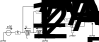
\includegraphics[width=0.6\linewidth]{electronique_soustracteur1.pdf}
\end{figure}

\begin{enumerate}

\item Pour pour connaitre la position de l'électroaimant, on souhaite connaitre $\delta L$ en utilisant les tensions $u_1$ et $u_2$ aux bornes des bobines $L_1$ et $L_2$. 

Déterminer les tensions $u_1$ et $u_2$ en fonction de $e(t)$, $R$, $L_1$ et $L_2$.

\item Pour accéder à $\delta L$, on utilise le montage soustracteur suivant :

\begin{figure}[!h]
\centering
\includegraphics[width=0.6\linewidth]{electronique_soustracteur2.pdf}
\end{figure}

\begin{enumerate}

 \item Déterminer la tension $u_s$ de sortie en fonction de $u_A$ et $u_B$ et montrer qu'il s'agit d'un montage soustracteur.
 
 \item Comment relier le montage soustracteur à l'électroaimant de sorte à avoir $u_s=u_1-u_2$ (c'est-à-dire $u_A=u_1$ et $u_B=u_2$) ? Préciser comment choisir les résistances $R_A$ et $R_B$.
 
 \item On suppose que le montage précédent est réalisé, c'est-à-dire que $u_s=u_1-u_2$. Exprimer alors la fonction de transfert $H$ de l'ensemble sous la forme :
 \begin{align*}
 H(\omega)=\frac{u_s}{e}=H_0\frac{j\omega/\omega_0}{1+j\omega/\omega_0}
\end{align*}  
où $\omega_0$ et $H_0$ sont des fonctions de $L_e$, $R$ et $\delta \omega$.	

\item Tracer le diagramme de Bode de $H(\omega)$. Dequel type de filtre s'agit-il ? Dans quel gamme de fréquence doit-on se placer pour avoir une sorte indépendante de la fréquence et proportionnel à $\delta L$ ?

\end{enumerate}

\end{enumerate}

\newpage

\begin{correction}

\begin{enumerate}

\item On commence par $u_2$, qui est le plus simple à calculer (pont-diviseur) :
\begin{align*}
	u_2=\frac{jL_2\omega}{j(L_1+L_2)\omega + R}e
\end{align*}
Pour $u_1$, il faut tenir compte qu'il s'agit de la tension aux bornes de la bobines (et non par rapport à la masse). Le pont diviseur donne donc :
\begin{align*}
	u_1&=\frac{jL_1\omega}{jL_1\omega+R}(e-u_2) \\
	&=\frac{jL_1\omega}{jL_1\omega+R}\times\frac{jL_1\omega+R}{j(L_1+L_2)\omega + R}e\\
	&=\frac{jL_1\omega}{j(L_1+L_2)\omega + R}e
\end{align*}
\item

\begin{enumerate}

 \item Une loi des noeuds à l'entrée $+$ donne : $u_A=2u_+$, à l'entrée $-$ : $u_s+u_B=2u_-$. On a donc $u_s=u_1-u_2$.
 
 \item Il faut prendre au garde que les tensions $u_1$ et $u_2$ sont prises aux bornes des bobines et non par rapport à la masse, contrairement aux tensions du soustracteur. Il faut réaliser le montage suivant pour avoir la tension $u_1-u_2$ à la sortie du montage :
 
\includegraphics[width=0.9\linewidth]{electronique_soustracteur3.pdf}

D'autre part, pour éviter que la mesure des tensions ne perturbe le circuit de l'électroaimant, on prend les résistances $R_A$ et $R_B$ très grades devant $R$, $L_1\omega$ et $L_2\omega$.
 
 \item On a :
 \begin{align*}
 	H(\omega)=&\frac{u_1-u_2}{e} \\
 	=&\frac{j(L_1-L_2)\omega}{j(L_1+L_2)\omega+R}\\
 	=&\frac{L_1-L_2}{L_1+L_2}\frac{j\omega(L_1+L_2)/R}{1+j\omega(L_1+L_2)/R}
 \end{align*}
 On a donc $\omega_0=(L_1+L_2)/R=2L_e/R$ et $H_0=(L_1-L_2)/(L_1+L_2)=\delta L/L_e$.

\item Filtre passe-haut (cf diagramme de Bode du cours). On doit se placer dans une gamme de fréquence $\omega\gg\omega_0$, à ce moment là $H\simeq \delta L/L_e$.

\end{enumerate}

\end{enumerate}

\end{correction}
\chapter{Thermodynamique (sup)}

\newpage

\section{Chute d'une masse sur un piston $\bullet\bullet\bullet\circ$}

On considère un gaz parfait, de coefficient $\gamma$, à la température $T_0$, contenu dans un cylindre de section $S$ surmonté d'un piston, situé à une hauteur $a$ par rapport au fond du dispositif. Le piston, de masse négligeable, peut coulisser sans frottement et toutes les parois sont isolées thermiquement de l'extérieur, où la pression et la température sont respectivement $P_0$ et $T_0$. Le champ de gravitation est modélisé par la constante d'accélération $g$.

\begin{figure}[h!]
\centering
  \includegraphics[width=0.8\textwidth]{thermo_sable.pdf}
\end{figure}

Au dessus du piston, à une altitude $H$ (repérée par rapport au fond du cylindre), se trouve un sac de sable de masse totale $M$. On souhaite étudier dans un premier temps le cas où le sac de sable tombe d'un bloc sur le piston (shcéma de gauche), et puis la situation où la totalité du sable se déverse grain par grain sur le piston (schéma de droite).

\begin{enumerate}

\item Dans ce cas-là, on considère que le sac de sable tombe d'un bloc sur le piston.

\begin{enumerate}

\item A quel type de transformation a t-on affaire dans ce cas-là ? Décrire qualitativement ce qu'il se passe.

\item Calculer la hauteur $x$ finale du piston après le retour à l'équilibre.

\item En déduire qu'il existe une hauteur $H_c$ critique à laquelle le piston remonte, à la suite du choc, à la même hauteur initiale $a$. Donner son expression et décrire qualitativement ce qu'il se passe si $H<H_c$ ou $H>H_c$.

\end{enumerate}

\item On suppose désormais que le sac est percé d'un petit trou, laissant sortir les grains de sables les uns après les autres.

\begin{enumerate}

\item A quel type de transformation a t-on affaire dans ce cas-là ? Quelle différence avec le cas précédent ?

\item Quel est le déplacement $dx$ du piston après la chute d'un grain de sable de masse $dm$ ?

\item Calculer la hauteur $x$ finale du piston une fois tout le sable tombé dessus. Comparer cette expression avec celle trouvée précedemment et commenter.

\end{enumerate}

\end{enumerate}

\newpage

\begin{correction}

\begin{enumerate}

\item

\begin{enumerate}

\item C'est une transformation brutale. Les paramètres du gaz dans le cylindre ne sont pas définis durant cette transformation ; on ne peut considérer que les états initiaux et finaux. Il va y avoir échauffement du gaz car l'énergie potentielle de la masse sera transférée sous forme de chaleur, ainsi que sous le travail des forces de pression extérieur.

\item Etat inital du gaz : $(P,T,V) =(P_0,T_0,aS)$. Etat final : $(P,T,V) =(P_f,T_f,xS)$ (3 inconnues, il faut donc trois équations). L'équilibre mécanique implique : $P_f=P_0+Mg/S$. L'équation des gaz parfait et le premier principe permettent d'obtenir deux autres équations indépendantes. 

Le premier principe appliqué au système {masse $M$ ; gaz} donne :
\begin{align*}
	\Delta U + \Delta E_p &= W \\
	\frac{nR}{\gamma-1}(T_f-T_0)+Mg(x-H)=&-P_0S(x-a)
\end{align*}
On précise que la variation d'énergie interne de la masse $M$ et d'énergie potentielle du gaz sont négligeable. D'autre part, $Q=0$ car pas d'échange thermique avec l'extérieur. Enfin, le travail de pression se fait à \textbf{pression extérieure constante} $P_0$ donc $W=-P_0S(x-a)$. En utilisant la loi des GP, on trouve :
\begin{align*}
	x(P_0S+Mg)=\frac{\gamma-1}{\gamma}MgH+P_0Sa
\end{align*}

\item On a retour à la hauteur initiale si $x=A$, alors $H_c=\frac{\gamma}{\gamma-1}a$. Si $H<H_c$, le piston s'enfonce plus bas que $a$ : l'énergie du choc ne dégage pas assez d'énergie thermique pour soulever le poids du sac. Si $H>H_c$, le piston s'élève par rapport à $a$.

\end{enumerate}

\item

\begin{enumerate}

\item C'est une transformation que l'on peut considérer comme inifiniment lente, donc réversible : chaque grain de sable faisant que très légèrement bouger le piston. Les paramètres du gaz sont constamment définis.

\item On utilise le même raisonnement que précédemment. On considère une transformation $(T,P,V)\longrightarrow(T+dT,P+dP,V+dV$ après la chute d'un grain de sable de masse $dm$. On a : $dP=gdm/S$ (équilibre des pressions) et $dV=Sdx$.
Premier principe :
\begin{align*}
	\frac{nRdT}{\gamma-1}+dmg(x-H)=&-P_0Sdx
\end{align*}
Or la loi des gaz parfaits donne :
\begin{align*}
& (P+dP)(V+dV)=nr(T+dT) \\
\Rightarrow \quad & P_0Sdx+dmgx=nRdT
\end{align*}
(ce qui revient différencier cette loi). 
On a donc :
\begin{align*}
P_0Sdx=dmg\left(\frac{\gamma-1}{\gamma}H-x \right) 
\end{align*}
\textit{NB} : on retrouve bien le résultat de la question précédente, avec $dx$ positif ou négatif si $H$ supérieur ou inférieur à $H_c$.

\item Il faut intégrer la relation précédente. En posant la variable intermédiaire $u=\frac{\gamma}{\gamma-1}\frac{x}{H}$, on trouve :
\begin{align*}
 \int_{\frac{\gamma}{\gamma-1}\frac{a}{H}}^{\frac{\gamma}{\gamma-1}\frac{x}{H}}\frac{du}{1-u}=\frac{Mg}{P_0S}
\end{align*}
On trouve alors :
\begin{align*}
x=\frac{\gamma-1}{\gamma}H(1-e^{-\frac{Mg}{P_0S}})+ae^{-\frac{Mg}{P_0S}}
\end{align*}

\end{enumerate}

\end{enumerate}

\end{correction}

\newpage	

\section{Entropie d'une chute libre $\bullet\bullet\bullet\circ$}

On considère un gaz parfait, de coefficient $\gamma$, à la température $T_0$, contenu dans un cylindre de section $S$ surmonté d'un piston, situé à une hauteur $a$ par rapport au fond du dispositif. Le piston, de masse négligeable, peut coulisser sans frottement et toutes les parois sont isolées thermiquement de l'extérieur, où la pression et la température sont respectivement $P_0$ et $T_0$. Le champ de gravitation est modélisé par la constante d'accélération $g$.

\begin{figure}[h!]
\centering
  \includegraphics[width=0.3\textwidth]{thermo_sable_bis.pdf}
\end{figure}

On fait tomber un grain de sable de masse $dm$ sur le cylindre, d'une hauteur $H$.

\begin{enumerate}

\item A quel type de transformation a t-on affaire ?

\item Quel est le déplacement $dx$ du piston après la chute d'un grain de sable de masse $dm$ ?

\item En déduire la variation d'entropie du gaz $dS_g$ lors de cette transformation. On rappelle que, pour un gaz parfait de $n$ moles, la variation d'entropie lors d'une transformation élémentaire s'écrit :
\begin{align*}
	dS=\frac{nR}{\gamma-1}\left(\frac{dP}{P}+\gamma\frac{dV}{V} \right) 
\end{align*}

\item En déduire que l'entropie créée par la chute d'une masse $M$ d'une hauteur $H$ à la température $T_0$ s'écrit :
\begin{align*}
	s_c=\frac{MgH}{T_0}
\end{align*} 

\end{enumerate}

\newpage

\begin{correction}

\begin{enumerate}

\item Cf exercice précédent. C'est une transformation que l'on peut considérer comme inifiniment lente, donc réversible : chaque grain de sable faisant que très légèrement bouger le piston. Les paramètres du gaz sont constamment définis.

\item Cf exercice précédent :
\begin{align*}
P_0Sdx=dmg\left(\frac{\gamma-1}{\gamma}H-x \right) 
\end{align*}

\item Avec la formule donnée :
\begin{align*}
	dS_g&=\frac{nR}{\gamma-1}\left(\frac{dP}{P}+\gamma\frac{dV}{V} \right) \\
	&=\frac{nR}{\gamma-1}\left(\frac{dmg}{SP_0}+\gamma\frac{dx}{x} \right) \\
	&=dm\frac{nRg}{(SP_0}\left(\frac{H}{x}-1 \right)
\end{align*}
Or, $nR/P_0=V_0/T_0=Sx/T_0$, donc :
\begin{align*}
	dS_g&=dm\frac{g}{T_0}(x-H)
\end{align*}
Pour une masse $M$ au lieu de $dm$, on obtient le résultat escompté. 

\item La variation d'entropie du système {gaz ; $M$} s'écrit :
\begin{align*}
	dS = dS_g+dS_M=\delta s_c + \delta s_e
\end{align*}
Comme il n'y a pas de transferts thermiques, $\delta s_e=0$. D'autre part, l'entropie de la masse $M$ ne change pas car il reste à tempréature constante. Lors de cette transofmration on a donc :
\begin{align*}
	s_c=\frac{MgH}{T_0}
\end{align*} 

\end{enumerate}

\end{correction}

\newpage

\section{Machine de Stirling $\bullet\bullet\circ\circ$}

On considère une machine thermodynamique, constituée d'un cylindre dans lequel coulisse un piston, qui effectue les transformations suivantes sur $n$ moles gaz parfait de coefficient $\gamma$ : 

\begin{itemize}
\item[$A \rightarrow B$ :] compression isotherme du volume $V_A$ au volume $V_B$, réversible, à la température $T_f$ (contact avec une source froide) ;
\item[$B \rightarrow C$ :] échauffement isochore ;
\item[$C \rightarrow D$ :] détente isotherme de $V_B$ à $V_A$, réversible à la température $T_c$ (contact avec une source chaude) ;
\item[$D \rightarrow A$] : refroidissement isochore.

\end{itemize}

Le cycle de Stirling a l'avantage de pouvoir être réalisable en pratique sur des dispositifs appelés \textit{moteurs de Stirling}, contrairement au cycle de Carnot, théorique.

\begin{enumerate}

	\item Décrire ce cycle dans un diagramme de Clapeyron $(P,V)$ et justifier qu'il est moteur.

	\item Déterminer, pour chaque transformation, $\Delta U$, $W$, et $Q$ en fonction de températures de la source chaude et de la source froide et du rapport de compression $a=V_A/V_B$.
	
	\item  Calculer son rendement $\eta$, et montrer qu'il est nécessairement inférieur au rendement de Carnot $\eta_C$.
	
	\item Avec un système appelé regénérateur, il est possible de stocker momentanément la chaleur évacuée de $D \rightarrow A$, pour la retransférer durant la transformation $B \rightarrow C$. Calculer le rendement $\eta'$ avec ce dispositif.
		
\end{enumerate}

\newpage

\begin{correction}

\begin{enumerate}

	\item Facile à représenter. Le cycle est moteur car il tourne dans le sens horaire donc l'intégrale $W=-\oint PdV<0$

	\item Pour le calcul du travail pour une transformation isotherme, on a :
		\begin{align*}
	W = -\int_i^f P\dif V &= nRT\ln\left(\frac{V_i}{V_f} \right) 
\end{align*}
	\begin{center}
\begin{tabular}{|p{2,5cm}|p{3cm}|p{3cm}|p{3cm}|}
\hline
Transformation & $\Delta U$ & $W$ & $Q$ \\
\hline
$A\rightarrow B$ & 0  & $nRT_f\ln a$  & $-nRT_f\ln a$  \\
\hline
$B\rightarrow C$ & $\frac{nR}{\gamma-1}(T_c-T_f)$ & 0 & $\frac{nR}{\gamma-1}(T_c-T_f)$  \\
\hline
$C\rightarrow D$ & 0  & $-nRT_c\ln a$ & $nRT_c\ln a$ \\
\hline
$D\rightarrow A$ & -$\frac{nR}{\gamma-1}(T_c-T_f)$ & 0 & -$\frac{nR}{\gamma-1}(T_c-T_f)$ \\
\hline
\end{tabular}
\end{center}
	
	\item  La chaleur apportée par souce chaude est $Q_c=Q_{C\rightarrow D}+Q_{B\rightarrow C}$. Le rendement $\eta$ est donc
	\begin{align*}
		\eta&=\frac{-W}{Q_c}=\frac{nR(T_c-T_f)\ln a}{\frac{nR}{\gamma-1}(T_c-T_f)+nRT_c\ln a} \\
		&=\frac{T_c-T_f}{T_c+\frac{T_c-T_f}{\ln(a)(\gamma-1)}}
	\end{align*}
	Or le rendement de Carnot est $\eta_C=\frac{T_c-T_f}{T_c}$ : ce dernier est supérieur car le dénominateur de la fraction est inférieur.
	
	\item Dans ce cas-là, le rendement devient :
	\begin{align*}
		\eta&=\frac{-W}{Q_c-Q_{B\rightarrow C}}=\frac{nR(T_c-T_f)\ln a}{nRT_c\ln a} \\
		&=\frac{T_c-T_f}{T_c} \\
		&=\eta_C
	\end{align*}	
		
\end{enumerate}

\end{correction}

\newpage

\section{Cycle de Beau de Rochas $\bullet\bullet\circ\circ$}

Les moteurs à essence équipant la plupart des véhicules terrestres sont des machines thermodynamiques généralement constitués de plusieurs cylindres, dans lequels un piston fait subir sur $n$ moles de gaz parfait le cycle suivant (dit de Beau de Rochas) :

\begin{itemize}

\item[$A \rightarrow B$ :] compression adiabatique, réversible du volume $V_A$ au volume $V_B$ : le mélange d'air frais et essence est comprimé ;
\item[$B \rightarrow C$ :] échauffement isochore en contact de la source chaude, en pratique il s'agit de la combustion très rapide de l'essence dégageant une chaleur $Q_c$ ;
\item[$C \rightarrow D$ :] détente adiabatique, réversible du volume $V_B$ au volume $V_C=V_A$ : les gaz de combustion "poussent" le cylindre en fournissant du travail ;
\item[$D \rightarrow A$ :] refroidissement isochore en contact de la source froide : les gaz issus de combustion sont évacués et remplacés par par un mélange d'air frais et d'essence. Le cycle reprend ensuite.

\end{itemize}

Ce cycle de fonctionnement a l'avantage de pouvoir faire varier la puissance du moteur très rapidement, car il est facile de contrôler la quantité de chaleur $Q_c$ apportée par la combustion de l'essence lors de la transformation $B \rightarrow C$. On souhaite montrer que cet avantage pratique se fait néanmoins au détriment du rendement $\eta$, qui est nécessairement inférieur au rendement de Carnot $\eta_C$.

\begin{enumerate}

	\item Décrire ce cycle dans un diagramme de Clapeyron $(P,V)$ et justifier qu'il est moteur.

	\item Déterminer, pour chaque transformation, $\Delta U$, $W$, et $Q$ en fonction de températures $T_A$, $T_B$, $T_C$ et $T_D$ atteintes aux moments $A$, $B$, $C$ et $D$.
	
	\item Exprimer les températures $T_B$, $T_C$ et $T_D$ à partir de $T_A=300$K, la température de l'air ambiant, et de $Q_c$, la chaleur dégagée par la combustion d'essence. Pour simplifier l'écriture, on pourra utiliser le taux de compression $a=V_A/V_B$.
	
	\item  Calculer son rendement $\eta$ en fonction de $a$ et $\gamma$, et montrer qu'il est nécessairement inférieur au rendement de Carnot $\eta_C$.
	
	%\item Calculer l'entropie crée $s_c$ sur un cycle. Commenter.
	
\end{enumerate}

\newpage

\begin{correction}

\begin{enumerate}

	\item Facile à représenter. Le cycle est moteur car il tourne dans le sens horaire donc l'intégrale $W=-\oint PdV<0$

	\item On peut proposer d'effectuer le calcul suivant pour le calcul du travail :
	\begin{align*}
	W = -\int_i^f P\dif V &= -cste\int_i^f \frac{\dif V}{V^{\gamma}}\\
	&=-cste\frac{V_f^{1-k}-V_i^{1-k}}{1-k}\\
	&=\frac{P_fV_f-P_iV_i}{\gamma-1}\\
	&= \frac{nR}{\gamma-1}(T_f-T_i)
\end{align*}
Appliquer le premier principe suffit aussi. On utilise le résultat précédent pour les transformations $A\rightarrow B$ et $D\rightarrow A$. Pour les transformations isochores, on calcule $\Delta U$ tout simplement pour l'échauffement d'un gaz.

\begin{center}
\begin{tabular}{|p{2,5cm}|p{3cm}|p{3cm}|p{3cm}|}
\hline
Transformation & $\Delta U$ & $W$ & $Q$ \\
\hline
$A\rightarrow B$ & $\frac{nR}{\gamma-1}(T_B-T_A)$  & $\frac{nR}{\gamma-1}(T_B-T_A)$  & 0  \\
\hline
$B\rightarrow C$ & $\frac{nR}{\gamma-1}(T_C-T_B)$ & 0 & $Q_c=\frac{nR}{\gamma-1}(T_C-T_B)$  \\
\hline
$C\rightarrow D$ & $\frac{nR}{\gamma-1}(T_D-T_C)$  & $\frac{nR}{\gamma-1}(T_D-T_C)$ & 0 \\
\hline
$D\rightarrow A$ & $\frac{nR}{\gamma-1}(T_A-T_D)$ & 0 & $Q_f=\frac{nR}{\gamma-1}(T_A-T_D)$ \\
\hline
\end{tabular}
\end{center}

\item On détermine la température à chaque transformation :
\begin{itemize}
	\item[$A\rightarrow B$ :] $T_B=a^{\gamma-1}T_A$ car compression adabatique en utilisant $TV^{\gamma-1}=cste$.
	\item[$B\rightarrow C$ :] $T_C=\frac{nR}{\gamma-1}Q_c + T_B$, d'après le premier principe : on échauffe le gaz en lui apportant $Q_c$.
	\item[$C\rightarrow D$ :] $T_D=T_C/a^{\gamma-1}$ car compression adabatique.
\end{itemize}


 \item  Pour calculer le rendement, il faut expliciter la quantité de chaleur $Q_c$ issue de la source chaude : il s'agit de $Q_{AB}$, car on augmente la pression à volume constant, c'est-à-dire qu'on apporte de la chaleur. Ici, elle est apportée par l'explosion de l'essence. Le travail total sur un cycle, quant à lui, s'écrit :

\begin{align*}
	W &= -\frac{nR}{\gamma-1}(T_B-T_A+T_D-T_C)\\
	&=-\frac{nR}{\gamma-1}(T_D-T_A) + Q_c
\end{align*}
On a donc :
\begin{align*}
	T_D = \frac{\gamma-1}{a^{\gamma-1}nR}Q_c+T_f
\end{align*}

Donc $W=Q_c\left( 1-\frac{1}{a^{\gamma-1}}\right) $ et alors :
\begin{align*}
	\eta= 1-\frac{1}{a^{\gamma-1}}
\end{align*}

	Pour comparer avec le rendement de Carnot $\eta_C=1-T_f/T_c$, il faut expliciter les températures de la source chaude $T_c$ et froide $T_f$. La température de la source chaude est à priori $T_C$ car le gaz est au maximum de sa température en $C$. En effet, comme la transformation $C\longrightarrow D$ est réversible, elle est supposée très lente, donc on peut supposer que le gaz s'est thermalisé à la température de la source chaude en $C$. 
	
	A ce moment là :
	\begin{align*}
		\eta_C&=1-\frac{T_A}{T_C}\\
		&=1-\frac{T_A}{\frac{\gamma-1}{nR}Q_c+a^{\gamma-1}T_A}\\
		&=1-\frac{1}{\frac{\gamma-1}{nRT_A}Q_c+a^{\gamma-1}}\\
		&>1-\frac{1}{a^{\gamma-1}} = \eta
	\end{align*}

On retrouve bien le fait que le rendement de Carnot est supérieur.

\end{enumerate}

\end{correction}

\newpage

\section{Compression brutale $\bullet\bullet\circ\circ$}

On considère le dispositif ci-dessous : un piston pouvant coulisser librement dans un cylindre, tous deux ayant des parois adiabatiques. Une paroi interne sépare les espaces $A$ et $B$ est fixe et diatherme et est percée d'un trou fermé par une fenêtre amovible. La pression extérieure est $P_0=1$ bar. Initialement, le volume $A$ est rempli d'une mole de gaz parfait $\gamma=1,4$, avec une pression $P_0=1$ bar, une température $T_0=300$K, tandis que le volume $B$ est vide.

\begin{figure}[!h]
\centering
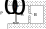
\includegraphics[width=0.5\linewidth]{thermo_pistonAB.pdf}
\end{figure}

\begin{enumerate}
\item On ouvre la fenêtre. Décrire qualitativement ce qu'il se passe suivant le volume de $A$ et $B$. En déduire l'existence d'un volume critique $V_C$ pour le volume $A$, que l'on ne demande pas de calculer ici.

\item On suppose $V_A<V_C$. Déterminez l'état final du gaz : on exprimera $V_f$ en fonction de $V_B$, $T_f$ en fonction de $T_0$ et $P_f$ en fonction de $P_0$. En déduire $V_C$.

\item Calculer la création d'entropie. Quelle est la cause de la création d'entropie ? On rappelle que lors d'une transformation $(P_i,T_i)\rightarrow  (P_f, T_f)$ sur $n$ moles de gaz parfait, on a :
\begin{align*}
	\Delta_i^f S=\frac{nR\gamma}{\gamma-1}\ln\left(\frac{T_f}{T_i} \right) - nR\ln\left(\frac{P_f}{P_i} \right)
\end{align*}

\item On suppose désormais que $V_A>V_C$. Quel est l'état final ?

\end{enumerate}

\newpage

\begin{correction}

\begin{enumerate}

\item Si $V_A\gg V_B$, alors tout le gaz se répartit dans $B$ sans que le piston ne touche la paroi interne. Inversement, si $V_A\ll V_B$, le piston va venir se coller contre la paroi interne et le gaz va intégralement dans $B$. Il y a donc une situation intermédiaire "limite" entre les deux où le piston va doucement se coller contre la paroi interne mais avec une équilibre des pressions.

\item Dans ce cas-là, le piston se colle contre la paroi : on a donc $V_f=V_B$. Il faut considérer le système {gaz+vide dans $B$} lorsqu'on applique le premier principe, avec donc $V_i=V_A+V_B$. Alors, comme la transformation est brutale, on a :
\begin{align*}
	\frac{nR}{\gamma-1}(T_f-T_0)&=W \\
	&=-P_0(V_f-V_i) \\
	&=-P_0V_A
\end{align*}
Avec la loi des gaz parfaits, appliqué sur le gaz contenu en $A$, on a $P_0V_A=nRT_0$, on trouve donc :  $T_f=\gamma T_0$ et $P_f=\gamma P_0V_A/V_B$.

Le volume critique est donc lorsqu'il y a équilibre des pressions : $P_0=P_f$, soit $V_A=V_C=V_B\gamma$.


\item Il n'y a pas d'échange de chaleur, donc $S_e=0$, alors $\Delta S=S_c$. On trouve :
\begin{align*}
	S_c=\Delta_i^f S=\frac{nR\gamma}{\gamma-1}\ln\left(\gamma \right) - nR\ln\left(\gamma\frac{V_A}{V_B} \right)
\end{align*}
L'entropie créée est bien positive, car on a $V_A<V_C$. Dans ce cas limite, on a $S_c=-nR\ln(\gamma-1)>0$.


\item On suppose désormais que $V_A>V_C$. Quel est l'état final ?

\end{enumerate}

\end{correction}

\newpage

\section{Compresseur à deux étages $\bullet\bullet\circ\circ$}

Pour de nombreux usages, on souhaite obtenir de l'air comprimé, c'est-à-dire de l'air à la température ambiante $T_0=300$K mais à une pression $P_1$ plus élevée que la pression atmosphérique $P_0=1$ bar, généralement $P_1=8$ bars. On notera $a=P_1/P_0$ le rapport de compression voulu.

\begin{enumerate}

\item On dispose dans un premier temps d'un cylindre muni d'un piston amenant $n$ moles de gaz parfait  (de coefficient $\gamma$) de l'état $(P_0, T_0)$ à l'état $(P_1, T_0)$ selon le chemin suivant :
\begin{itemize}

	\item[$A\rightarrow B$ :] compression adiabatique et réversible de $(P_0, T_0)$ à $(P_1, T_1)$ ;
	\item[$B\rightarrow C$ :] refroidissement isobare de $T_1$ à $T_0$.
	
\end{itemize}

Le refroidissement se fait avec une thermalisation avec l'atmosphère ambiant qui reste à $T_0$.

\begin{enumerate}

\item Représenter la transformation $(P_0, T_0)\rightarrow (P_1, T_0)$ dans un diagramme de Clapeyron.
\item Calculer le travail $W$ fourni par le piston durant cette transformation, en fonction de $P_0$, $V_0$ et de $a$. 
\item Calculer l'entropie créée $s_c$ et commenter.

\end{enumerate}

\item On souhaite diminuer le travail $W$ fourni pour comprimer le gaz. Pour cela, on comprime le gaz en deux temps, en ajoutant un étage de compression (en pratique un second cylindre à la suite du premier). La transformation du gaz est désormais :
\begin{itemize}

	\item[$A\rightarrow B$ :] compression adiabatique et réversible de $(P_0, T_0)$ à $(P_i, T_i)$ ;
	\item[$B\rightarrow C$ :] refroidissement isobare de $T_i$ à $T_0$ ;
	\item[$C\rightarrow D$ :] compression adiabatique et réversible de $(P_i, T_0)$ à $(P_1, T_1)$ ;
	\item[$D\rightarrow E$ :] refroidissement isobare de $T_1$ à $T_0$.
	
\end{itemize}

\begin{enumerate}

\item Représenter cette nouvelle transformation $(P_0, T_0)\rightarrow (P_1, T_0)$ dans un diagramme de Clapeyron.
\item Calculer le travail $W'$ fourni par le piston, en fonction de $P_0$, $V_0$, $P_1$ et $P_i$.
\item Comment doit-on choisir $P_i$ pour minimiser le travail fourni ? En déduire $W'$ pour cette valeur de $P_i$ et montrer que $W'<W$.
\item Calculer l'entropie créée $s_c'$. Comparer avec $s_c$ et commenter.

\end{enumerate}

\item Quelle serait la transformation pour que le travail fourni soit minimal ? Justifier à l'aide d'un diagramme de Clapeyron. Pourquoi est-ce difficilement réalisable en pratique ? Calculer alors l'entropie créée.

\end{enumerate}

On rappelle que lors d'une transformation $(P_i,T_i)\rightarrow  (P_f, T_f)$ sur $n$ moles de gaz parfait, on a :
\begin{align*}
	\Delta_i^f S=\frac{nR\gamma}{\gamma-1}\ln\left(\frac{T_f}{T_i} \right) - nR\ln\left(\frac{P_f}{P_i} \right)
\end{align*}

\newpage

\begin{correction}

\begin{enumerate}

\item

\begin{enumerate}

\item Pour le diagramme de Clapeyron, on peut passer du volume à la température avec la loi des gaz parfaits.

\centering
\includegraphics[width=0.5\linewidth]{thermo_cor_compresseur.png}


\item Le travail de $A\rightarrow B$ est $\frac{nR}{\gamma-1}(T_B-T_0)=\frac{(P_1V_B-P_0V_0)}{\gamma-1}$, et celui de $B\rightarrow C$ est $-P_1(V_1-V_B)$. En utilisant la loi de Laplace, on a $V_B=V_0(P_0/P_1)^{1/\gamma}$. Le travail total est donc :
\begin{align*}
	W=\frac{\gamma P_0V_0}{\gamma-1}\left(a^{\frac{\gamma-1}{\gamma}}-1 \right) 
\end{align*}

\item On a $\Delta S=\frac{nR\gamma}{\gamma-1}\ln\left( \frac{T_0}{T_1}\right)$, car transformation isentropique sur $AB$ et isobare sur $BC$. L'entropie échangée se fait à la température extérieure $T_0$, elle s'écrit :
\begin{align*}
	s_e &= \frac{Q}{T_0} \\
	&=\frac{nR\gamma}{\gamma-1}\frac{T_0-T_1}{T_0}
\end{align*}
car $Q=\frac{nR\gamma}{\gamma-1}(T_0-T_1)$ sur $BC$. 
L'entropie créée est donc :
\begin{align*}
	s_c & = \Delta S - s_e \\
	&=\frac{nR\gamma}{\gamma-1}\left[\frac{T_1}{T_0}-1-\ln\left( \frac{T_1}{T_0} \right) \right] 
\end{align*}
Celle-ci est bien positive car $x-1<\ln x$. En fonction de $a$, elle s'exprime :
\begin{align*}
	s_c =\frac{nR\gamma}{\gamma-1}\left[a^\frac{\gamma-1}{\gamma}-1-\frac{\gamma-1}{\gamma}\ln\left( a \right) \right] 
\end{align*}
en utilisant que $P^{1-\gamma}T^\gamma$ est constant sur $AB$.

\end{enumerate}

\item 

\begin{enumerate}

\item Cf le diagramme à la première question.

\item On additionne les travaux effetués. Comme les transformations $ABC$ et $CDE$ sont les mêmes, on peut utiliser les mêmes expression du travail que trouvé précédemment. On obtient :
\begin{align*}
	W'=&\frac{\gamma P_0V_0}{\gamma-1}\left[\left( \frac{P_i}{P_0}\right) ^{\frac{\gamma-1}{\gamma}}-1 \right] +\frac{\gamma P_iV_i}{\gamma-1}\left[\left( \frac{P_1}{P_i}\right) ^{\frac{\gamma-1}{\gamma}}-1 \right] \\
	=&\frac{\gamma P_0V_0}{\gamma-1}\left[\left( \frac{P_i}{P_0}\right) ^{\frac{\gamma-1}{\gamma}}+\left( \frac{P_1}{P_i}\right) ^{\frac{\gamma-1}{\gamma}}-2 \right] 
\end{align*}
\item On calcule $dW'/dP_i=0$. Aorès des calculs plus ou moins laborieux, on trouve $P_i=\sqrt{P_0P_1}$. Le travail s'exprime alors :
\begin{align*}
	W'=\frac{2\gamma P_0V_0}{\gamma-1}\left(a^{\frac{\gamma-1}{2\gamma}}-1 \right) 
\end{align*}
En posant $x=a^{\frac{\gamma-1}{2\gamma}}$, on a :
\begin{align*}
 W-W'=&\frac{\gamma P_0V_0}{\gamma-1}\left(x^2-1-2(x-1) \right) \\
 =&\frac{\gamma P_0V_0}{\gamma-1}(x^2-2x+1) \\
 =&\frac{\gamma P_0V_0}{\gamma-1}(x-1)^2\\
 &>0 
\end{align*}
Le travail est donc inférieur lorsque le compresseur a deux étages.
 
\item Avec un calcul similaire à celui du travail (il y a le log en plus), on trouve :
\begin{align*}
		s_c =\frac{2nR\gamma}{\gamma-1}\left[a^\frac{\gamma-1}{2\gamma}-1-\frac{\gamma-1}{2\gamma}\ln\left( a \right) \right] 
\end{align*}
Pour montrer que l'entropie créee est alors inférieur à la précédente, même raisonnement que la question précédente, en posant $x=a^{\frac{\gamma-1}{2\gamma}}$ :
\begin{align*}
	s_c'-s_c&=\frac{nR\gamma}{\gamma-1}\left(x^2-1-2(x-1) \right) \\
	=&\frac{\gamma nR}{\gamma-1}(x-1)^2\\
 &>0 
\end{align*}

\end{enumerate}

\item Comme on souhaite augmenter la pression tout en finissant à la même température, on peut imaginer vers cela avec une isotherme. Un diagramme de Claperon permet rapidement de voir que la travail à fournir est plus faible que les transformrations précédentes. Difficile à réaliser en pratique car une compression adiabatique réversible est beaucoup plus rapide qu'une thermalisation isotherme.

L'entropie créée dans ce cas-là est nulle, car l'entropie échangée est égale à la variation d'entropie.

\end{enumerate}

\end{correction}

\newpage

\section{Puissance d'une arme à feu $\bullet\bullet\bullet\bullet$}

On considère le canon d'une arme à feu, constitué d'un tube de diamètre $d$ et de longueur $L$, dans peut glisser sans frottement une balle (le projectile). Au coup de feu, la poudre contenue dans le volume $Sx_0$ (en pointillé) explose et dégage instantanément une énergie $Q$. La balle, de masse $m$, initialement emboitée sur la cartouche en $x_0$, est alors propulsée dans le canon, dont les parois sont supposées adiabatiques.

\begin{figure}[h!]
\centering
  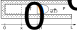
\includegraphics[width=0.65\textwidth]{thermo_fusil.pdf}
\end{figure}

On pourra modéliser le mélange d'air et de gaz issu de la combustion comme un gaz parfait de coefficient $\gamma$, à la pression $P$ et à la température $T$ lorsque le projectile est à l'abscisse $x$. Pour le calibre 5.56 OTAN, on donne : $Q\approx5000$ J, $x_0$=110 mm et $d=5,56$ mm.

\begin{enumerate}

	\item Estimer la pression $P_1$ juste après la combustion et montrer que pour des valeurs raisonnable de $L$, la pression atmosphérique $P_0$ est toujours négligeable devant $P$.
	
	\item Montrer que la vitesse de la balle en sortie de canon s'écrit :
	\begin{align*}
		v_m=\sqrt{\frac{2Q}{m}}\sqrt{1-\left(\frac{L}{x_0} \right)^{1-\gamma}}
	\end{align*}
	
	\item Calculer la pression $P_m$ et la température $T_m$ du gaz lorsque la balle sort du canon. Commenter.

\end{enumerate}
\chapter{Thermodynamique (spé)}

\newpage

\section{Premier principe sur un fluide en écoulement stationnaire $\bullet\circ\circ\circ$}

Préciser les hypothèses et établir l'expression générale du premier principe pour un fluide en écoulement stationnaire à travers une machine quelconque sous la forme (les grandeurs thermodynamiques massiques sont en minuscule) :
\begin{align*}
	\Delta (h+e_p+e_c)=w_u+q
\end{align*}
Préciser la signification physique de chacun des termes et son unité.
Même question, en faisant apparaître le débit massique du fluide $D_m$ :
\begin{align*}
	D_m\Delta (h+e_p+e_c)=P_u+P_{th}
\end{align*}

\newpage

\section{Second principe sur un fluide en écoulement stationnaire $\bullet\circ\circ\circ$}

Préciser les hypothèses et établir l'expression générale du second principe pour un fluide en écoulement stationnaire à travers une machine quelconque sous la forme (les grandeurs thermodynamiques massiques sont en minuscule) :
\begin{align*}
	\Delta s=s_{ech}+s_{créée}
\end{align*}
Préciser la signification physique de chacun des termes et son unité.
Même question, en faisant apparaître le débit massique du fluide $D_m$ :
\begin{align*}
	D_m\Delta s=\dot{S}_{ech}+\dot{S}_{créée}
\end{align*}

\newpage

\section{Pompe de relevage $\bullet\circ\circ\circ$}

Une pompe de relevage est une machine remontant un fluide de masse volumique $\rho$ d'un dénivelé $h$. On supposera que les sections d'entrée et de sortie du fluide sont identiques. 

\begin{enumerate}

	\item Préciser les hypothèses et établir l'expression générale du premier principe pour un fluide en écoulement stationnaire à travers une machine quelconque sous la forme (les grandeurs thermodynamiques massiques sont en minuscule) :
\begin{align*}
	\Delta (h+e_p+e_c)=w_u+q
\end{align*}
Préciser la signification physique de chacun des termes et son unité.
	\item Même question, en faisant apparaître le débit massique du fluide $D_m$ :
\begin{align*}
	D_m\Delta (h+e_p+e_c)=P_u+P_{th}
\end{align*}
	
	\item Lors du passage dans la machine, y a t-il variation d'énergie cinétique, potentielle ou thermique ?
	
	\item Exprimer la puissance de la pompe $p$ pour relever le fluide avec un débit massique $d$. 
	
	\item Rappeler les densités typiques d'un gaz et d'un liquide. Ce type de machine est-il couramment utilisé pour relever des gaz ou des liquides ?

\end{enumerate}

\newpage

\begin{correction}

\begin{enumerate}

	\item Il n'y a uniquement que de la variation d'énergie potentielle ; les sections d'entrée et de sortie étant identiques, il n'y a pas de variation d'énergie cinétique ; une pompe ne chauffe pas, donc pas de variation de température.
	
	\item On applique le premier principe industriel :
	\begin{align*}
		dgh = p
	\end{align*}
	
	\item Densité d'une phase condensée : $\rho\simeq1-8\times10^3$kg/m$^3$, d'un gaz : $\rho\simeq1\times$kg/m$^3$. On l'utilise pour les liquides.

\end{enumerate}

\end{correction}

\newpage

\section{Ecoulement d'un torrent}

Un torrent s'écoule sur une montagne sur un dénivelé de 1000m, du fait de sa viscosité et des turbulences, la vitesse reste constante lors de son trajet. Pour simplifier, on suppose que l'écoulement est adiabatique car suffisament rapide pour pouvoir négliger les tranferts thermiques. 

\begin{enumerate}

\item

\begin{enumerate}

	\item Calculer l'échauffement de l'eau lors de sa descente. La capacité calorifique de l'eau est $c_P=4$kJ/K/kg. 
	
\end{enumerate}

\item On souhaite comparer de ce qui, entre l'air et l'eau, s'échauffe le plus lors de la descente en montagne. On suppose aussi qu'un écoulement d'air decend sur le même dénivelé de manière adiabatique et réversible. 

\begin{enumerate}

	\item Montrer que la variation d'enthalpie massique de l'air peut s'écrire :
	\begin{align*}
		\Delta h =\frac{\gamma R}{M(\gamma -1)}\Delta T
	\end{align*}
	où $M=29$g/mol est la masse molaire de l'air.

	\item Comparer avec la différence de température de l'air entre le haut et le bas de la montagne. Qui s'échauffe le plus entre l'eau et l'air ?
	
	\item Quelle est la variation d'entropie massique de cet écoulement d'air ? 
	
\end{enumerate}

\end{enumerate}

\newpage

\begin{correction}

\begin{enumerate}

\item On applique le premier principe industriel : $c_p\Delta T+g\Delta z=0$. On trouve que $\Delta T = 0,25$ K, ce qui est très faible : l'eau ne s'échaufe que très peu.

\item On rappelle que la variation d'entropie de $n$ moles de gaz s'écrit $\Delta H=\frac{nR\gamma}{\gamma-1}\Delta T$

\end{enumerate}

\end{correction}

\newpage

\section{Compresseur}

Un compresseur augmente la pression d'un gaz parfait arrivant au débit massique $d_m$ de $P_1$ à $P_2$, on notera $a=P_2/P_1$ le taux de compression. La section dans laquelle circule le gaz est supposé constante. On suppose dans un premier temps que la compression est adiabatique et réversible.

\begin{enumerate}

\item

\begin{enumerate}

	\item Citer deux exemples d'objet utilisant un compresseur à flux continu.
	
	\item Quelle est la température $T_2$ du gaz en sortie du compresseur ?
	
	\item En déduire le travail massique $w_u$ nécessaire pour comprimer ce gaz. Exprimer aussi la puissance $p_u$ de ce compresseur.

\end{enumerate}

\item

On suppose désormais que les pertes thermiques sont importantes : la compression n'est plus adiabatique, elle est isotherme. 

\begin{enumerate}

	\item Quelle est le travail massique $w_u$ nécessaire pour comprimer ce gaz dans ce cas-là ? En déduire la chaleur massique $q$ perdue par le gaz. 
	
	\item Calculer la variation d'entropie massique $\Delta s$ du gaz lors de la compression.
	
\end{enumerate}

\end{enumerate}

\newpage

\section{Tuyère}

Une tuyère est un dispositif utilisé dans l'aérospatiale, dans laquelle un gaz chaud issu d'une combustion est accéléré en se refroidissant : elle convertit l'énergie thermique du gaz en énergie cinétique, servant à la propulsion d'un engin. Une tuyère (représentée ci-dessous, avec un profil divergent $(1)$ et un profil convergent $(2)$) est un conduit de symétrie de révolution selon l'axe $Ox$, de section variable ($S(x)$ à l'abscisse $x$), dont les parois sont calorifugées, sans aucune pièce mécanique à l'intérieur.

\begin{figure}[!h]
\centering
	
\includegraphics[width=0.9\linewidth]{thermo_tuyere.pdf}
\end{figure}

Les gaz issus de la combustion, de capacité calorifique $c_P$, sont, en $x=0$, à la température $T_0$ et à la vitesse $v_0$. On note $T(x)$ et $v(x)$ la température et la vitesse du gaz à l'abscisse $x$. On formule les hypothèses suivantes :
\begin{itemize}
	\item Le gaz est très chaud à l'entrée de la tuyère et sa vitesse faible, c'est-à-dire que $\frac{1}{2}v_0^2\ll c_PT_0$ ; 
	\item La section $S(x)$ varie lentement de sorte que la vitesse du gaz est orthogonale en tout point de la section $S(x)$ ;
	\item La vitesse du gaz est toujours inférieure à celle du son.
\end{itemize}

\vspace{1cm}

A partir de ces hypothèses, la tuyère doit-elle avoir un profil divergent $(1)$ ou convergent $(2)$ pour que les gaz soient accélérés ?

\newpage

\begin{correction}

Il faut déterminer la température et la vitesse dans la tuyère. Le premier principe industriel s'écrit :
\begin{align*}
	\frac{1}{2}v^2(x)+c_PT(x)=\frac{1}{2}v^2_0+c_PT_0
\end{align*}
Pour obtenir une nouvelle équation sur $T$, on peut utiliser la loi de Laplace, qui s'écrit :
\begin{align*}
T(x)\rho(x)^{1-\gamma}=T_0\rho_0^{1-\gamma}
\end{align*}
où $\rho$ est la masse volumique du gaz. Avec la conservation du débit massique, on obtient une dernière équation :
\begin{align*}
	D_m=\rho(x)v(x)S(x)=\rho_0v_0S_0
\end{align*}
En injectant dans l'équation du premier principe, on obtient :
\begin{align*}
	\frac{1}{2}v^2(x)+c_PT_0\left( \frac{v(x)S(x)}{v_0S_0}\right)^{1-\gamma}=\frac{1}{2}v^2_0+c_PT_0
\end{align*}
On introduit la quantité $u(x)=v(x)/v_0$, $\sigma(x)=S(x)/S_0$ et $\eta_0=2c_PT_0/v_0^2$. D'après les hypothèses de l'énoncé, $\eta_0\ll1$. Alors :
\begin{align*}
	u^{\gamma+1}(x)+\eta_0\sigma^{1-\gamma}(x)=(1+\eta_0)u^{\gamma-1}(x)
\end{align*}
On a donc une équation permettant de connaitre directement la vitesse en fonction de la section, même s'il faut tout de même un petit coup de main numérique pour avoir le profil exact. Néanmoins, on peut ruser pour savoir s'il faut un profil divergent ou convergent, en dérivant cette équation :
\begin{align*}
	(\gamma+1)u'(x)u^{\gamma}(x)+(1-\gamma)\eta_0\sigma'(x)\sigma^{-\gamma}(x)=(1+\eta_0)(\gamma-1)u'(x)u^{\gamma-2}(x)
\end{align*}
Et alors :
\begin{align*}
	u'(x)=\frac{1}{(\gamma+1)u^{\gamma}(x)-(1+\eta_0)(\gamma-1)u^{\gamma-2}(x)}\times(\gamma-1)\eta_0\sigma^{-\gamma}(x)\times\sigma'(x)
\end{align*}
Il faut étudier le signe du dénominateur de la fraction. On peut le factoriser par $(\gamma+1)u^{\gamma-2}(x)$ pour obtenir :
\begin{align*}
	u^{2}(x)-(1+\eta_0)\frac{\gamma-1}{\gamma+1}&= \frac{2}{v_0^2}\left[\frac{1}{2}v^{2}(x)-\frac{\gamma-1}{\gamma+1}\left( \frac{1}{2}v^{2}_0+c_PT_0\right) \right] \\
	&<0
\end{align*}
Ce terme est négatif car $c_pT_0\gg \frac{1}{2}v^{2}_0$, \textit{a fortiori}, même avec le facteur $\frac{\gamma-1}{\gamma+1}\simeq 0,17$, tant que le gaz n'a pas encore accéléré, le terme thermique reste supérieur. Il faut donc que la dérivée $\sigma'(x)<0$ pour que $u'(x)>0$ : les gaz accélèrent.

\end{correction}

\subsubsection*{Turbine à gaz}

\subsubsection*{Echangeur}

\newpage

\section{Formation du brouillard $\bullet\circ\circ$}

On considère un gaz parfait de coefficient $\gamma$ contenu dans un cylindre de section $S$ orienté verticalement. L'altitude le long de ce cylindre est notée $z$, et on note $g$ l'accélération de la pesanteur supposée uniforme le long du cylindre. Le gaz est soumis à un mouvement ascendant dans le cylindre en se déplaçant à la vitesse notée $c$. Les parois du cylindre ne permettent pas de transfert thermique. L'écoulement est de plus supposé stationnaire.

On note $T_0$, $P_0$ et $c_0$ la température, la pression et la vitesse du gaz à l'altitude $z=0$ et $T(z)$, $P(z)$ et $c(z)$ ces trois grandeurs à l'altitude $z$. De la même manière, on introduit $h_{m,0}$ et $h_m(z)$ l'enthalpie massique du gaz à l'altitude $z=0$ et $z$.

\begin{enumerate}

\item

\begin{enumerate}
	
	\item En utilisant le premier principe industriel appliqué au gaz dans le cylindre entre les altitudes $z=0$ et $z$, trouver une relation entre $h_{m,0}$, $h_m(z)$, $c_0$, $c(z)$ et $z$.
	
	\item Pour simplifier le problème, on considère que la vitesse du gaz est quasi-nulle, de sorte à ce que $c_0=c(z)=0$. Montrer que la température obéit alors à la loi suivante :
	\begin{align*}
		T(z)=T_0\left( 1-\frac{z}{H}\right) 
	\end{align*}
	Expliciter $H$ en fonction de $\gamma$, $g$ et la masse molaire du gaz $M$. Donner une estimation numérique.
	
\end{enumerate}

\item On considère que le gaz étudié est de l'air humide, subissant une ascension verticale, lente et isentropique dans ce cylindre. La vapeur d'eau contenue en faible quantité dans l'air se comporte comme un gaz parfait. La pression de vapeur saturante de l'eau, notée $P_s$ et exprimée en Pa est une focntion de $T$ suivant la loi empirique suivante :
\begin{align*}
	\ln(P_s(T)) = a -\frac{b}{T}
\end{align*}

\begin{enumerate}
	
	\item Soit $\varphi$ la fraction molaire de vapeur d'eau contenue dans une masse d'air ascendante. Après avoir explicité la pression $P(z)$ dans la colonne, déterminer la pression partielle $P_e(z)$ de cette vapeur. 
	
	\item A quelle altitude, notée $z_1$, peut-on avoir le changement d'état liquide-vapeur ? On pourra supposer que $z\ll H$.
	
	\item Justifier que les reliefs sont propices à l'apparition du brouillard.
	
\end{enumerate}

\end{enumerate}

\newpage	

\section{Etude d'un turborécteur $\bullet\bullet\circ\circ$}

Un turboréacteur est un moteur thermique équipant les avions dits \textit{à réaction}, schématisé ci-dessous. Le fonctionnement général est le suivant : un turbine aspire et comprime l'air en amont du réacteur (étape $1\rightarrow2$), qui est ensuite chauffé par la combustion du kérosène dans la chambre de combustion (étape $2\rightarrow3$). Les gaz de combustion sont alors détendus ($3\rightarrow4$) à travers une turbine dont l'arbre est commun avec celui du compresseur, puis ces gaz sont finalement évacués par la tuyère ($4\rightarrow5$), en accélérant fortement, fournissant la poussée requise.

Le but de l'exercice est de calculer la vitesse de sortie $c_5$ des gaz de combustion, fournissant la poussée à l'aéronef.

\begin{figure}[!h]
\centering
	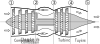
\includegraphics[width=0.8\linewidth]{thermo_turboreacteur.pdf}
\end{figure}

On formule les hypothèses suivantes pour les différentes transformations :
\begin{itemize}

	\item[$1\rightarrow2$ :] Compresseur, compression adiabatique réversible au taux de compression $a=P_2/P_1=26$ ;
	\item[$2\rightarrow3$ :] Chambre de combustion, le gaz est chauffé jusqu'à $T_3=1450$K de manière isobare ;
	\item[$3\rightarrow4$ :] Détente adiabatique réversible du gaz de $P_3$ et $P_4$ à travers la turbine ;
	\item[$5\rightarrow6$ :] Détente adiabatique réversible du gaz de $P_4$ et $P_5$ dans la tuyère.

\end{itemize}

On supposera que le régime est stationnaire, que l'énergie potentielle de pesanteur du fluide est négligeable dans toutes les étapes. L'énergie cinétique sera aussi négligée dans toutes les étapes, sauf à la sortie de la tuyère (en 5) où le gaz est très fortement accéléré. On négligera tout frottement mécanique. Les pressions en entrée et en sortie sont $P_1=P_5=1$ bar et la température en entrée est $T_1=288$K. On note $C_p$ la capacité thermique massique de l'air.

\begin{enumerate}

	\item En utilisant un bilan de masse et d'énergie, montrer que le travail massique utile reçu par le gaz lors d'une transformation de l'état $i$ à $j$ (sauf pour $2\rightarrow3$, dans la chambre de combustion) est donné par :
	\begin{align*}
		w_{i\rightarrow j}=C_p(T_j-T_i) + \frac{1}{2}\left(c_j^2-c_i^2 \right) 
	\end{align*}
	\item Donner une relation entre $P_i$, $P_j$, $T_i$, $T_j$ et $\gamma$ (sauf pour $2\rightarrow3$).
	\item En exploitant le couplage mécanique entre la turbine et le compresseur, établir les expressions littérales et les valeurs numériques des températures $T_2$, $T_4$ et de la pression $P_4$ en sortie de turbine.
	\item En déduire la vitesse $c_5$ à la sortie du réacteur. 
	\item \textit{(PSI, PC)} En déduire la poussée du réacteur en kN.

\end{enumerate}

\textit{Données :} $C_p=1,0\times10^3$J.kg$^{-1}$.K$^{-1}$, $\gamma=1,4$

\newpage

\section{Etude d'un turborécteur $\bullet\bullet\bullet\bullet$}

Un turboréacteur est un moteur thermique équipant les avions dits \textit{à réaction}, schématisé ci-dessous. Le fonctionnement général est le suivant : un turbine aspire et comprime l'air en amont du réacteur (étape $1\rightarrow2$), qui est ensuite chauffé par la combustion du kérosène dans la chambre de combustion (étape $2\rightarrow3$). Les gaz de combustion sont alors détendus ($3\rightarrow4$) à travers une turbine dont l'arbre est commun avec celui du compresseur, puis ces gaz sont finalement évacués par la tuyère ($4\rightarrow5$), en accélérant fortement, fournissant la poussée requise.

Le but de l'exercice est de calculer la vitesse de sortie $c_5$ des gaz de combustion, fournissant la poussée à l'aéronef.

\begin{figure}[!h]
\centering
	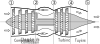
\includegraphics[width=0.8\linewidth]{thermo_turboreacteur.pdf}
\end{figure}

On formule les hypothèses suivantes pour les différentes transformations :
\begin{itemize}

	\item[$1\rightarrow2$ :] Compresseur, compression adiabatique réversible au taux de compression $a=P_2/P_1=26$ ;
	\item[$2\rightarrow3$ :] Chambre de combustion, le gaz est chauffé jusqu'à $T_3=1450$K de manière isobare ;
	\item[$3\rightarrow4$ :] Détente adiabatique réversible du gaz de $P_3$ et $P_4$ à travers la turbine ;
	\item[$5\rightarrow6$ :] Détente adiabatique réversible du gaz de $P_4$ et $P_5$ dans la tuyère.

\end{itemize}

On supposera que le régime est stationnaire, que l'énergie potentielle de pesanteur du fluide est négligeable dans toutes les étapes. L'énergie cinétique sera aussi négligée dans toutes les étapes, sauf à la sortie de la tuyère (en 5) où le gaz est très fortement accéléré. On négligera tout frottement mécanique. Les pressions en entrée et en sortie sont $P_1=P_5=1$ bar et la température en entrée est $T_1=288$K. On rappelle que la masse molaire de l'air est $M=29$g.mol$^{-1}$. 

\vspace{1cm}

Calculer la vitesse d'éjection $c_5$ des gaz à la sortie de la tuyère et en déduire la poussée que peut fournir ce turboréacteur.

\newpage

\begin{correction}

\begin{enumerate}

	\item Il s'agit simplementde la démonstration du premier principe industriel appliqué sur une transformation $i\rightarrow j$ (à demander dans la question).
	
	\item On utilise la loi de Laplace, valide pour toutes les transformations sauf lors de la combustion (l'hypothèse adiabatique n'est plus valide) :
	\begin{align*}
		P_1^{1-\gamma}T_1^\gamma&=P_2^{1-\gamma}T_2^\gamma \\
		P_3^{1-\gamma}T_3^\gamma&=P_4^{1-\gamma}T_4^\gamma \\
		P_4^{1-\gamma}T_4^\gamma&=P_5^{1-\gamma}T_5^\gamma \\
	\end{align*}
	
	\item Avec le rapport de compression $a$: 
	\begin{align*}
		T_2=&T_1a^{\frac{\gamma-1}{\gamma}} \\
		=&731K
	\end{align*}
	Ensuite, on utilise le couplage mécanique de l'arbre entre la turbine et le compresseur : $w_{1\rightarrow2}=C_p(T_2-T_1) =-w_{3\rightarrow}=C_p(T_4-T_3)$
	On a alors :
	\begin{align*}
		T_4=& T_3-(T_2-T_1)\\
		=& T_3-T_1\left(a^\frac{\gamma-1}{\gamma}-1 \right) \\
		=&907\mathrm{K}
	\end{align*}
	Pour la pression $P_4$, on utilise la transformation isobare dans la chambre de combustion :
	\begin{align*}
		P_4&=P_3\left(\frac{T_3}{T_4} \right)^\frac{\gamma}{1-\gamma}\\
		&=aP_1\left(\frac{T_3}{T_4} \right)^\frac{\gamma}{1-\gamma} \\
		&=6,5 \mathrm{bars}
	\end{align*}
	Et enfin pour $T_5$ :
	\begin{align*}
		T_5&=T_4\left(\frac{P_4}{P_5} \right) ^{\frac{\gamma-1}{\gamma}} \\
		&=T_3a^{\frac{1-\gamma}{\gamma}}\\
		&=532\mathrm{K}
	\end{align*}
	
	\item Avec le premier principe industriel, on a :
	\begin{align*}
		c_5=&\sqrt{2C_p(T_4-T_5)} \\
		=&866\mathrm{m.s}^{-1}
	\end{align*}
	
	
\end{enumerate}

\end{correction}
\include{diffusion}
\chapter{Mécanique}

\newpage

\section{Le Petit Prince : satellisation d'une pomme $\bullet\bullet\circ\circ$}

On se place à la surface d'une planète de rayon $R$ et de champ gravitationnel $g$. On envoie une pomme avec une vitesse $v_0$ purement horizontale et on négligera les frottements de l'air.

\begin{enumerate}
\item En supposant la planète localement plane, déterminer la hauteur d$z$ dont est tombée la pomme après avoir parcouru une longueur d$x$ dans le plan horizontal. % d$z=\dfrac{g(\mathrm{d}x)^2}{2{v_0}^2}$
\item Après une distance horizontale d$x$, de combien le sol de la planète est-il descendu ? On pourra utiliser les formules pour les petits angles : $\tan\theta\simeq \theta$, $\sin\theta\simeq \theta$ et $\cos\theta\simeq 1-\theta^2/2$. % Il faut penser à la rotondité de la Terre qui n'est donc pas parfaitement plane localement : d$h=R-R\cos(\mathrm{d}\theta)=R(\mathrm{d}\theta)^2/2=(\mathrm{d}x)^2/2R$
\item En déduire qu'il existe une certaine vitesse $v_0$ pour laquelle la pomme va revenir à son point de départ. % v_0=\sqrt{GM/R}$
\end{enumerate}

\newpage

\begin{correction}

\begin{enumerate}
\item La planète étant supposée parfaitement plane, on peut commencer par calculer l'équation du mouvement de la pomme. Soumise à la seule force de pesanteur, on obtient :

\begin{align*}
	\left\lbrace
\begin{array}{ccc}
 x(t) =  v_0t+x_0 \\
 z(t) = -\frac{1}{2}gt^2+z_0 \\
\end{array}\right.
\end{align*}
En supposant que $x_0$ et $z_0$ sont les coordonnées de la position initiale. On obtient donc l'équation de la trajectoire :
\begin{align*}
	z(x) = -\frac{g(x-x_0)^2}{2v_0^2}+z_0
\end{align*}

Lorsque la pomme avance de $dx$ par rapport à sa position initiale $x_0$, elle descend de $z_0$ à $z_0+dz$ :
\begin{align*}
	z(x_0+dx)=z_0+dz=-\frac{gdx^2}{2v_0^2}+z_0
\end{align*}
Donc $dz=-\frac{gdx^2}{2{v_0}^2}$.

\item Il faut penser à la rotondité de la Terre qui n'est donc pas parfaitement plane localement : d$h=R-R\cos(\mathrm{d}\theta)=R(\mathrm{d}\theta)^2/2=(\mathrm{d}x)^2/2R$.

\item Si la vitesse initiale est suffisament grande, la chute de la pomme est compensée par le fait que le sol "s'abaisse" en même temps à cause de la rotondité, cad $dh=-dz$, soit $v_0=\sqrt{gR}=\sqrt{GM_T/R}$.

\item Si la pomme revient à son point de départ, c'est que la trajectoire est supposée circulaire, avec $R$ constant. On peut effectuer un PFD sur la pomme en coordonnées cylindriques, et trouver à partir de la projection sur $\vec{e}_r$ :

\begin{align*}
 -mR\dot{\theta}^2 =  -\frac{GmM_T}{R^2} 
\end{align*}
Soit $v_0=R\dot{\theta}=\sqrt{GM_T/R}$.
\end{enumerate}

\end{correction}

\newpage

\section{Projectile lancé à la verticale $\bullet\circ\circ\circ$}

On tire un petit projectile à la verticale, avec une vitesse initiale $v_0$. Le problème est de calculer son altitude $z$ en fonction du temps, en tenant compte de la gravité et de la résistance de l'air. Comme l'objet est petit, on supposera que la résistance de l'air est proportionnelle à la vitesse et que la force de résistance est $m\gamma v$, $m$ étant la masse de l'objet, $v$ sa vitesse et $\gamma$ une constante. Nous supposerons que la force de gravité est constante (on néglige sa variation en fonction de l'altitude). On adoptera comme origine la position du tir ($z=0$) et on supposera que le mouvement ne se produit que dans la direction $z$.

\begin{enumerate}
\item Soit $v(t)$ la composante en $z$ de la vitesse du projectile. \'{E}crivez l'équation différentielle que doit satisfaire $v(t)$ en fonction du temps, d'après la deuxième loi de Newton.
\item Résoudre cette équation différentielle avec la condition initiale $v(0)=v_0$.
\item Exprimer maintenant l'altitude $z$ en fonction du temps.
\item Calculer l'altitude maximale atteinte par le projectile ($z_\mathrm{max}$), en fonction des paramètres $v_0$, $g$ et $\gamma$.
\item Exprimer le résultat de la question précédente ($z_\mathrm{max}$) dans les limites de très faible résistance ($\gamma \rightarrow 0$) et de très forte résistance ($\gamma \rightarrow \infty$). Quelles modifications mineures devrait-on apporter à l'équation différentielle trouvée première question pour retrouver ces résultats plus simplement ?

\end{enumerate}

\newpage

\begin{correction}

\begin{itemize}
\item Rien de bien difficile, en notant $v=\dot{z}$ :

\begin{align*}
	m\dot{v}=-\gamma mv-mg
\end{align*}

\item
La solution de cette équation est :
\begin{align*}
	v(t) = \left(v_0+\frac{g}{\gamma} \right)\exp\left(-\gamma t\right)-\frac{g}{\gamma}  
\end{align*}

\item On intègre l'expression de la vitesse précédente. On trouve :

\begin{align*}
	z(t) = \frac{1}{\gamma}\left(v_0+\frac{g}{\gamma} \right) \left(1-\exp(-\gamma t) \right) -\frac{g}{\gamma}t
\end{align*}
\item L'altitude maximale correspond à l'instant $t_0$ où la vitesse s'annule : $v(t_0)=0$, soit $t_0 = \frac{1}{\gamma}\ln\left(\frac{1+v_0\gamma}{g} \right) $. On a donc :
$z_\mathrm{max}=\frac{v_0}{\gamma}-\frac{g}{\gamma^2}\ln\left( 1+\frac{\gamma v_0}{g}\right).$

\item Dans le cas où $\gamma\rightarrow0$, $z_\mathrm{max}\rightarrow\frac{v_0}{\gamma}-\frac{g}{\gamma^2}\frac{\gamma v_0}{g}+\frac{g}{2\gamma^2}\frac{\gamma^2 v_0^2}{g^2}=\frac{ v_0^2}{2g}$ en utilisant $\ln(1+x)\simeq 1+x-x^2/2$. Cela correspond à une chute libre ne l'absence de frottement. 

Dans le cas où $\gamma\rightarrow0$, $z_\mathrm{max}\rightarrow\frac{v_0}{\gamma}$

\end{itemize}

\end{correction}

\newpage

\section{Paramètre d'impact $\bullet\bullet\circ\circ$}

Une météorite arrive depuis l'infini vers la Terre avec une vitesse à l'infini $\vec{v}_0$. La Terre a une masse $M_T$ et un rayon $R_T$. On note $b$ le paramètre d'impact comme indiqué sur la figure ci-dessous. L'objectif de ce problème est de déterminer la valeur minimale de $b$ pour laquelle la météorite évite la collision avec la Terre.

\begin{figure}[h]
\centering
  \includegraphics[scale=0.4]{meca_parametre_impact.png}
\end{figure}

\begin{enumerate}
\item La météorite n'est soumise qu'à la force gravitationnelle de la Terre. Déterminer la nature de sa trajectoire. Montrer que le mouvement est plan et déterminer une relation entre $r$ et $\dot{\theta}$.
\item On note $N$ le point de la trajectoire où la distance qui sépare la météorite de la Terre est la plus petite. Montrer qu'en $N$, la vitesse est uniquement suivant $\vec{u}_\theta$. Déterminer une relation entre $v_N$ au point $N$, la distance $ON$, $b$ et $v_0$.
\item En utilisant la conservation de l'énergie, montrer la relation :
$$
0=r^2_\mathrm{min}v_0^2+2GM_Tr_\mathrm{min}-v_0^2b^2.
$$
\item En déduire l'expression minimale $b_c$ du paramètre d'impact telle que pour $b<b_c$, la météorite frappe la Terre et pour $b>b_c$, la météorite évite la Terre. On pourra exprimer le résultat en fonction de la vitesse de libération $v_\mathrm{lib}$.
\end{enumerate}

\newpage

\begin{correction}

\begin{enumerate}
\item La météorite n'est soumise qu'à la gravitation, qui est une force centrale. On peut donc utiliser la conservation du moment cinétique (car le moment des forces est nul). Comme le moment se converve, il est dirigé ortohogonalement au plan délimité par $\vec{r_0}$ et $\vec{v_0}$ tout le long de la trajectoire. Le mouvement reste donc conscrit à ce plan.

D'autre part, on a par la conservation du moment :
\begin{align*}
	\vec{\sigma}_O(M)=m\vec{r}\wedge\vec{v}=-mr_0v_0sin(\theta_0)=-mbv_0
\end{align*}

Et d'autre part, $\vec{v}=\dot{r}\vec{e}_r+r\dot{\theta}\vec{e}_\theta$, donc $\vec{\sigma}_O(M)=r^2\dot{\theta}=-mbv_0$.


\item La distance $ON$ entre la météorite et la terre correspond à la coorodnnée $r$. Lorsque celle-ci est minimale, on a nécéssairement $\dot{r}=0$. La vitesse s'exprime donc $\vec{v}=\dot{r}\vec{e}_r+r\dot{\theta}\vec{e}_\theta=r\dot{\theta}\vec{e}_\theta$.

A ce point, le moment cinétique est $\vec{\sigma}_O=ON\cdot v_N$. Par conservation du moment on a alors :
\begin{align*}
	ON\cdot v_N=bv_0
\end{align*}

\item L'énergie potentielle de gravitation s'écrit $E_p=-GM_Tm/r^2$. L'énergie mécanqiue totale du système est égale au point $N$ et à l'infini (lorsque la météorite arrive à la vitesse $v_0$), alors :
\begin{align*}
	\frac{1}{2}mv_N^2-\frac{GM_Tm}{r_N}
\end{align*}
$$
0=r^2_\mathrm{min}v_0^2+2GM_Tr_\mathrm{min}-v_0^2b^2.
$$
\item En déduire l'expression minimale $b_c$ du paramètre d'impact telle que pour $b<b_c$, la météorite frappe la Terre et pour $b>b_c$, la météorite évite la Terre. On pourra exprimer le résultat en fonction de la vitesse de libération $v_\mathrm{lib}$.

\end{enumerate}

\end{correction}

\newpage

\section{Piège de Penning $\bullet\bullet\bullet\circ$}

A l'aide d'un dispositif approprié, on créé dans une région de l'espace au voisinage d'un point $O$ un champ électrique défini en coordonnées carthésiennes par :
\begin{align*}
	\vec{E}=\frac{U_0}{2R^2}\left(-x\vec{e}_x-y\vec{e}_y+2z\vec{e}_z \right) 
\end{align*}
Un électron de masse $m$ et de charge $e$ se meut dans la région située autour du point $O$.

\begin{enumerate}

	\item Montrer que le point $O$ est une position d'équilibre pour l'éléctron. Discuter de la stabilité selon les directions. On introduira $\omega_z^2=eU_0/mR^2$.

 \item Pour stabiliser la trajectoire de l'électron, on supperpose au champ électrique un champ magnétique uniforme et constant $\vec{B}=B_0\vec{e}_z$. On définit $\omega_c=eB_0/m$. 

\begin{enumerate}

		\item Montrer que le mouvement suivant $\vec{e}_z$ est inchangé.
		
		\item Pour le mouvement dans le plan $(xOy)$, montrer que l'électron n'est piégé que si $B_0$ est supérieur a une certaine valeur $B_c$, à déterminer en fonction des données de l'exercice. On utilisera le changement de variable : $\rho = x+iy$.
		
		\item Résoudre l'équation en $\rho$ pour le cas $B_0\gg B_c$, sans chercher à mettre en évidence les constante d'intégration, mais en mettant en évidence deux pulsations, l'une voisine de $\omega_c$, notée $\omega_c'$, et une autre notée $\omega_m$, appelée pulsation magnétique. 

\end{enumerate}
		
\end{enumerate}

\newpage

\begin{correction}

\begin{enumerate}

	\item On applique le principe fondamental de la dynamique à l'électron :
\begin{align*}
	\left\lbrace
\begin{array}{ccc}
 m\ddot{x} &=&  e\frac{U_0}{2R^2}x \\
 m\ddot{y} &=& e\frac{U_0}{2R^2}y \\
 m\ddot{z} &= & -e\frac{U_0}{R^2}z \\
\end{array}\right.
\end{align*}
La position est bien une position de stabilité : les forces appliquée en ce point sont nulles. Néanmoins, ce n'est pas une position stable en $x$ ou en $y$ car la solution est exponentielle. Le mouvement est stable uniquement sur $z$, avec une pulsation $\omega_z=eU_0/mR^2$.

\item

\begin{enumerate}

		\item Le PFD devient :
		
\begin{align*}
	\left\lbrace
\begin{array}{ccc}
 \ddot{x} &=&  \frac{\omega_z^2}{2}x - \omega_c\dot{y}\\
 \ddot{y} &=& \frac{\omega_z^2}{2}y + \omega_c\dot{x} \\
 \ddot{z} &= & -\omega_z^2z \\
\end{array}\right.
\end{align*}

Le mouvement selon $z$ est bien inchangé. 

		\item En multipliant la seconde première ligne par $i$, puis en sommant ces deux lignes, on obtient :
		\begin{align*}
 \ddot{\rho} - \frac{\omega_z^2}{2}\rho - i\omega_c\dot{\rho}=0\\
\end{align*}
		
		Le déterminant de l'équation caractéristique est $\Delta=2\omega_z^2-\omega_c^2$. Le mouvement est stable uniquement si $\Delta>0$, cad si $B_0>B_c=\sqrt{2mU_0/eR^2}$.
		
		\item Les solutions de l'équation caractéristiques sont :
		\begin{align*}
			r=i\frac{\omega_c}{2}\left( 1 \pm\sqrt{1- \frac{2\omega_z^2}{\omega_c^2}}\right) 
		\end{align*}
		
		Les pulsations caractéristiques sont donc $\omega_\pm=\frac{\omega_c}{2}\left( 1 \pm\sqrt{1- \frac{2\omega_z^2}{\omega_c^2}}\right)$. Dans le cas où $B_0\gg B_c$, $\omega_c\gg\omega_z$ et on peut donc écrire :
		\begin{align*}
			\omega_+&=\frac{\omega_c}{2}\left( 1 +\frac{\omega_z^2}{2\omega_c^2}\right)= \omega_c'\\
			\omega_-&=\frac{\omega_z^2}{2\omega_c}=\omega_m
		\end{align*}
		
		La solution est donc :
		\begin{align*}
			\rho(t)=Ae^{i\omega_c'}t+Be^{i\omega_mt}
		\end{align*}
		
		L'équation de la trajectoire est donnée par $x(t)=\mathrm{Re}(\rho(t))$ et $y(t)=\mathrm{Im}(\rho(t))$.

\end{enumerate}
		
\end{enumerate}

\end{correction}

\newpage

\section{Tir à grande distance $\bullet\bullet\circ\circ$}

Dans le jeu \textit{Call of Duty 4 : Modern Warfare}, le joueur prend le rôle d'un tireur d'élite devant abattre une cible située à une distance $d=$897m à l'aide d'un fusil de précision, qui tire un projectile à une vitesse $v_0=850$m.s$^{-1}$. Le tir s'effectue depuis le dernier étage d'un immeuble d'une hauteur $H=30$m, la cible se trouvant plein nord par rapport au tireur. La scène se situe en Russie, à une latitude $\lambda=45^\circ$. Le coéquipier du joueur précise, avant le tir, qu'il faut tenir compte de l'effet de Coriolis et l'on souhaite vérifier cette affirmation.

On définit $R=(O,x,y,z)$ le repère situé au pied de l'immeuble où se trouve le joueur, avec l'axe $\vec{e}_x$ dirigé vers l'est et l'axe $\vec{e}_y$ se dirigeant vers le nord. On notera $\vec{\Omega}_T$ le vecteur rotation de la terre. On supposera que les frottements de l'air sont négligés.

\begin{enumerate}

	\item Montrer que les équations du mouvement dans le référentiel $R$ de la balle une fois que le tireur fait feu s'écrivent :
	\begin{align*}
        \ddot{x}=&2\Omega_T(\sin\lambda\dot{y}-\cos\lambda\dot{z})\\ 
        \ddot{y}=&-2\Omega_T\sin\lambda\dot{x} \\
        \ddot{z}=&-g+2\Omega_T\cos\lambda\dot{x}
	\end{align*}
	
	\item Déterminer la solution sur $x(t)$ sans préciser les variables d'intégration.
	
	\item Donner une estimation du temps de vol avant impact $t_{impact}$ puis simplifier les équations du mouvement, les résoudre.
	
	\item Que pensez-vous de l'affirmation du coéquipier ? Quel est l'écart $\vec{\varepsilon}$ de la balle par rapport à si celle-ci avait une trajectoire parfaitement rectiligne ?

\end{enumerate}

\newpage

\section{Tir à grande distance $\bullet\bullet\bullet\bullet$}

Dans le jeu \textit{Call of Duty 4 : Modern Warfare}, le joueur prend le rôle d'un tireur d'élite devant abattre une cible située à une distance $d=$897m à l'aide d'un fusil de précision, qui tire un projectile à une vitesse $v_0=850$m.s$^{-1}$. Le tir s'effectue depuis le dernier étage d'un immeuble d'une hauteur $H=30$m, la cible se trouvant plein nord par rapport au tireur. La scène se situe en Russie, à une latitude $\lambda=45^\circ$. Le coéquipier du joueur précise, avant le tir, qu'il faut tenir compte de l'effet de Coriolis et l'on souhaite vérifier cette affirmation. On définit $R=(O,x,y,z)$ le repère situé au pied de l'immeuble où se trouve le joueur, avec l'axe $\vec{e}_x$ dirigé vers l'est et l'axe $\vec{e}_y$ se dirigeant vers le nord. On notera $\vec{\Omega}_T$ le vecteur rotation de la terre. On supposera que les frottements de l'air sont négligés.

Que pensez-vous de l'affirmation du coéquipier ? Quel est l'écart $\vec{\varepsilon}$ de la balle par rapport à si celle-ci avait une trajectoire parfaitement rectiligne ? On pourra donner une estimation du temps de vol avant impact $t_{impact}$ pour simplifier les équations du mouvement.

\newpage

\begin{correction}

On note $R'$ le référentiel du tireur, sur la terre en rotation, et $R$ le référentiel galiléen, ne tournant pas avec la terre. Le vecteur rotation de $R'/R$ s'écrit $\vec{\Omega}=\Omega_T\cdot(\cos\lambda\vec{e}_y+\sin\lambda\vec{e}_z)$ et on note le vecteur vitesse dans $R'$ : $\vec{v}=\dot{x}\vec{e}_x+\dot{y}\vec{e}_y+\dot{z}\vec{e}_z$. Une fois sortie du canon, la balle est uniquement soumise à la gravité et à la force de Coriolis (la force d'inertie d'entrainement est comprise dans $g$). Cette dernière s'écrit :
	\begin{align*}
		\vec{F}_c&=-2m\vec{\Omega}\wedge\vec{v} \\
		&=2m\Omega_T\left\lvert 
      \begin{matrix} 
        &\sin\lambda\dot{y}-\cos\lambda\dot{z}\\ 
        &-\sin\lambda\dot{x} \\
         &\cos\lambda\dot{x}
      \end{matrix}  
    \right.
	\end{align*}

Le PFD donne donc :
	\begin{align*}
        \ddot{x}=&2\Omega_T(\sin\lambda\dot{y}-\cos\lambda\dot{z})\\ 
        \ddot{y}=&-2\Omega_T\sin\lambda\dot{x} \\
        \ddot{z}=&-g+2\Omega_T\cos\lambda\dot{x}
	\end{align*}
Ces équations sont toutes intégrables. On intègre la deuxième et la troisième :
	\begin{align*}
        \ddot{x}=&2\Omega_T(\sin\lambda\dot{y}-\cos\lambda\dot{z})\\ 
        \dot{y}=&-2\Omega_T\sin\lambda x + \dot{y}_0 \\
        \dot{z}=&-gt+2\Omega_T\cos\lambda x + \dot{z}_0
	\end{align*}
Et on injecte dans la première équation sur $x$, et en simplifiant les $\cos^2+\sin^2$ : 
\begin{align*}
	\ddot{x}+4\Omega_T^2x=2\Omega_T(\sin\lambda\dot{y}_0-\cos\lambda\dot{z}_0)+2\Omega_T\cos\lambda gt
\end{align*}
	Cette équation est soluble : elle du genre $\ddot{x}+\omega_0^2=a+bt$. Néanmoins, la solution homogène en $\cos$ et $\sin$ n'est pas très intéressante : la période est celle de la journée terrestre, elle correspond en fait à ce que la balle fasse le tour de la Terre et revienne à sa position... Et en effet, comme $\Omega_T\simeq7,2\times10^{-7}$rad/s, on peut commencer à garder uniquement les termes en $\Omega_T^2$ d'ordre 1 devant les autres termes. On a donc, après simplification :
	\begin{align*}
        x(t)=& \frac{1}{3}\Omega_T\cos\lambda t^3+\Omega_T(\sin\lambda\dot{y}_0-\cos\lambda\dot{z}_0)t^2+\dot{x}_0t\\ 
        y(t)=&-\Omega_T\sin\lambda \dot{x}_0t^2 + \dot{y}_0t \\
        z(t)=&-\frac{1}{2} gt^2+\Omega_T\cos\lambda \dot{x}_0t^2 + \dot{z}_0t+z_0
	\end{align*}	
On a donc les équations du mouvement. Néanmoins, cela reste encore un peu dur de conclure. On peut encore essayer de simplifier certains termes, en utilisant l'estimation du temps de vol et la vitesse initiale. Le temps de vol, estimé à 1s environ, permet de comparer le premier et le deuxième terme dans l'équation sur $x(t)$ : $\frac{1}{3}gt^3\ll\dot{y}_0t^2$, durant tout le temps de vol, comme $\dot{y}_0\simeq 850$. D'autre part, comme le tir est dirigé plein nord, on a $\dot{x}_0=0$. On a alors :
	\begin{align*}
        x(t)=& \Omega_T(\sin\lambda\dot{y}_0-\cos\lambda\dot{z}_0)t^2\\ 
        y(t)=&\dot{y}_0t \\
        z(t)=&-\frac{1}{2} gt^2 + \dot{z}_0t+z_0
	\end{align*}	
Et en notant $\alpha$ l'angle que fait le tireur entre l'horizontale et la direction du canon (comme il est situé sur un immeuble, il y a un léger dénivellé entre lui et sa cible), on a :
	\begin{align*}
        x(t)=& v_0\Omega_T\sin(\lambda+\alpha)t^2\\ 
        y(t)=&v_0\cos(\alpha)t \\
        z(t)=&-\frac{1}{2} gt^2 -v_0\sin(\alpha)t+z_0
	\end{align*}	
Finalement, on se retrouve avec globalement une chute libre classique, si ce n'est un terme de déviation uniquement sur $x$, vers l'est. Si la balle partait de manière parfaitement rectiligne, sa trajectoire serait (soumise à aucune force) :
	\begin{align*}
        x'(t)=& 0\\ 
        y'(t)=&v_0\cos(\alpha)t \\
        z'(t)=& -v_0\sin(\alpha)t+z_0
	\end{align*}	
La dévitation est donc $\vec{\varepsilon	}=v_0\Omega_T\sin(\lambda+\alpha)t^2\vec{e}_x-\frac{1}{2} gt^2\vec{e}_z$. Pour un temps de vol d'environ 1 seconde, on trouve que :
\begin{align*}
	\vec{\varepsilon}=-0,5\vec{e}_z+0,04\vec{e}_x
\end{align*}
La balle est déviée de seulement 4cm vers l'est : Coriolis est donc négligeable. Par contre, il faut tenir compte du poids dont l'effet est bien plus marqué. 
	
\end{correction}

\newpage

\section{Frottement d'une corde et d'une poutre en bois $\bullet\bullet\circ\circ$}

Une corde est enroulée autour d'une poutre en bois de section circulaire, d erayon $R$, entre les angles $\theta_1$ et $\theta_2$. Au-delà de ces angles, la corde n'est plus en contact avec le bois et est soumise aux tensions $T_1$ et $T_2$ de part et d'autre de ses extrémités. Le coeffcient de forttement entre la corde et le bois est $f=0,5$. On note $T(\theta)$ la tension dans la corde à un angle $\theta$, c'est-à-dire la force qui s'exerce au sein de la corde.

\begin{figure}[h]
\centering
  
\includegraphics[scale=0.8]{meca_corde.pdf}
\end{figure}

\begin{enumerate}

	\item Montrer que la réaction normale $dR_N$ de la poutre sur un élément de longueur de corde $Rd\theta$ vérifie la relation suivante :
	\begin{align*}
		dR_N+T(\theta)d\theta=0
	\end{align*}
	
	\item Montrer que la réaction tangentielle $dR_T$ de la poutre sur un élément de longueur de corde $Rd\theta$ vérifie la relation suivante :
	\begin{align*}
		-dR_T+T(\theta+d\theta)-T(\theta)=0
	\end{align*}
	
	\item En déduire une équation différentielle sur la tension $T(\theta)$ et l'intégrer.
	
	\item Pour attacher son cheval, un cow-boy enroule tout simplement la longe de son cheval de plusieurs tour autour d'une poutre en bois de section ronde, puis laisse l'extrémité libre, soumise à son propre poids (environ 100g). Combien de tours le cow-boy doit-il effectuer pour qu ele cheval ne puisse pas dérouler la corde ?
	
\end{enumerate}

\textit{Indications} : la force maximale que peut développer un cheval est équivalent à une tonne ; le coefficient de frottement entre la corde et le bois est $f=0,5$.

\newpage

\section{Frottement d'une corde et d'une poutre en bois $\bullet\bullet\bullet\circ$}

Pour attacher son cheval, un cow-boy enroule tout simplement la longe de son cheval de plusieurs tour autour d'une poutre en bois de section ronde, puis laisse l'extrémité libre, soumise à son propre poids (environ 100g). Combien de tours le cow-boy doit-il effectuer pour qu ele cheval ne puisse pas dérouler la corde ?

\textit{Indications} : la force maximale que peut développer un cheval est équivalent à une tonne ; le coefficient de frottement entre la corde et le bois est $f=0,5$.
\chapter{Ondes mécaniques}

\newpage

\section{Longueur d'un son}

Une feuille métallique rectangulaire, de masse surfacique $\sigma=7,8\times10{-2}$kg.m$^{-3}$, de dimensions $l\times L=2\times2$m suivant les axes $x$ et $y$, est fixée sur un support le long des deux côtés de dimension $L=2$m. La feuille est tendue entre ces deux supports jusqu'à une tension $T_0=3,0\times10^6$N le long de l'axe $x$.

\begin{figure}[h]
\centering
  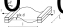
\includegraphics[scale=1.9]{onde_meca_feuille_vibrante.pdf}
\end{figure}

Lorsqu'on frappe sur cette plaque, on suppose qu'elle ne peut vibrer que suivant la direction $x$. Le son émis se propage à la vitesse $c_0=343$m.s$^{-1}$ dans l'air environnant dont la masse volumique est $\rho_0=1,3$kg.m$^{-3}$.

On frappe la plaque de sorte à ce que le son atteigne un volume sonore de 70dB à 1m de distance, durant les premiers instants. Estimer le temps au bout duquel le son ne sera plus perceptible.

\newpage

\begin{correction}

L'idée est de considérer la vibration mécanique de la feuille s'amortitissant en cédant de la puissance sonore à l'air, que l'on peut quantifier à partir du vecteur de Poynting sonore $\vec{Pi}$.

On commence par évaluer la fréquence de l'onde : $f\simeq c/\lambda$, où $\lambda\simeq 2l$ est la longueur d'onde du fondamental et $c$ la vitesse de l'onde mécanique dans la plaque, donnée par $c=\sqrt{T_0/\mu}=\sqrt{T_0/\sigma L}\simeq4,3\times10^3$m.s$^{-1}$. La plaque vibre donc à la fréquence $f\simeq 1,1$kHz, donc la longueur d'onde de l'onde sonore est $\lambda_0=c/f_0\simeq31$cm. On peut considérer que $\lambda_0 \ll L$, l'onde sonore est émise par un plan, donc est une onde "localement" plane. 

Avec la géométrie du problème, le champ de vitesse de cette onde peut s'écrire :
\begin{align*}
	\vec{v}(x,z,t)=\frac{d\psi}{dt}\left(x,t-\frac{z}{c}\right) \vec{e}_z
\end{align*}
car sur la surface de la feuille (le plan $z=0$), par conservation du débit, $\vec{v}(x,z=0,t)=\frac{d\psi}{dt}(x,t)$ où $\psi$ représente la hauteur de la vibration de la feuille par rapport à l'équilibre. Le champ de vitesse à une distance $z$ de la feuille est donc ensuite simplement décalé de $t-\frac{z}{c}$. 

La puissance propagée par l'onde sonore est donnée par le vecteur de Poynting $\vec{\Pi(x)}=p\vec{v}$. En $z=\psi$, cette puissance est :
\begin{align*}
	\vec{\Pi(x)}&=p(x,\psi,t)\vec{v}(x,\psi,t) \\
	&=Z_0v^2(x,\psi,t)\vec{e}_z \\
	&=Z_0\left( \frac{d\psi}{dt}\right)^2\vec{e}_z
\end{align*}
La puissance transmise à l'onde sonore est perdue par la plaque. Pour un élément de surface $dS=dx\times L$ de la feuille, la puissance cédée à l'onde sonore est :
\begin{align*}
	dP&=-||\vec{\Pi(x)}||dxL \\
	&=-Z_0dxL\left( \frac{d\psi}{dt}\right)^2 \\
	&=df_{frott.}\frac{d\psi}{dt}
\end{align*}
On peut écrire $dP$ comme la puissance cédée par l'élément de feuille $dx\times L$ se déplaçant à la vitesse $\frac{d\psi}{dt}$ par une force de frottement $df_{frott.}=-Z_0dxL\frac{d\psi}{dt}(x,t)$ :

On part maintenant sur l'analyse de la feuille. Pour un élément de feuille $dx\times L$, on peut appliquer le même raisonnement que pour le cas de la corde vibrante. Le PFD donne alors :
\begin{align*}
	\sigma dx  L\frac{d^2\psi}{dt^2}=-T(x)\sin\alpha(x)+T(x+dx)\sin\alpha(x+dx)-Z_0dxL\frac{d\psi}{dt}(x,t)
\end{align*}
On trouve alors, avec le raisonnement habituel de la corde vibrante :
\begin{align*}
	\frac{d^2\psi}{dt^2}=\frac{T_0}{\sigma L}\frac{d^2\psi}{dx^2} -\frac{Z_0}{\sigma}\frac{d\psi}{dt}(x,t)
\end{align*}
On notera $c^2=T_0/\sigma L$. On cherche alors des solutions stationnaires sous la forme $\psi(x,t)=f(x)g(t)$. En injectant dans l'équation précédente, et en divisant par $\psi(x,t)$, on obtient :
\begin{align*}
	\frac{g"(t)}{g(t)}+\frac{Z_0}{\sigma}\frac{g'(t)}{g(t)}=c^2\frac{f"(x)}{f(x)}
\end{align*}
La partie gauche de l'équation étant indépendante de $x$, on peut résoudre l'équation différentielle sur $f$. Avec les conditions aux limites, on trouve $f(x)=A\sin\left(\frac{n\pi x}{l}\right)$, avec $n\in\mathbb{Z}$. L'équation sur la fonction $g$ devient :
\begin{align*}
	g"(t)+\frac{Z_0}{\sigma}g'(t)+\frac{\pi^2n^2c^2}{l^2}=0
\end{align*}
La solution générale de cette équation est :
\begin{align*}
	g(t)=B\cos(\omega t +\phi)e^{-t/\tau}
\end{align*}
où $\tau=\frac{\sigma}{2Z_0}$.

\end{correction}
\include{optique}
\appendix
\chapter*{Appendix}
The first appendix text.

% ========================
%\backmatter
%\printbibliography
%\newpage
%\begin{center}
The back cover
\end{center}
\end{document}